%Copyright 2019 Christopher M. Jermaine (cmj4@rice.edu) and Risa B. Myers (rbm2@rice.edu)
%
%Licensed under the Apache License, Version 2.0 (the "License");
%you may not use this file except in compliance with the License.
%You may obtain a copy of the License at
%
%    https://www.apache.org/licenses/LICENSE-2.0
%
%Unless required by applicable law or agreed to in writing, software
%distributed under the License is distributed on an "AS IS" BASIS,
%WITHOUT WARRANTIES OR CONDITIONS OF ANY KIND, either express or implied.
%See the License for the specific language governing permissions and
%limitations under the License.
%===============================================================
\documentclass[aspectratio=169]{beamer}
\mode<presentation> 
{
\usetheme[noshadow, minimal,numbers,riceb,nonav]{Rice}
\usefonttheme[onlymath]{serif}
\setbeamercovered{transparent}
}
\useinnertheme{rectangles}

\usepackage[english]{babel}

\usepackage{amsmath}
\usepackage{mathptmx}
\usepackage{helvet}
\usepackage{courier}
\usepackage[T1]{fontenc}
\usepackage{trajan}
\usepackage{ textcomp }
\usepackage{listings}

\newenvironment{noindentitemize}
{ \begin{itemize}
 \setlength{\itemsep}{1.5ex}
  \setlength{\parsep}{0pt}   
  \setlength{\parskip}{0pt}
 \addtolength{\leftskip}{-2em}
 }
{ \end{itemize} }

\newenvironment{noindentitemize2}
{ \begin{itemize}
  \setlength{\itemsep}{0ex}
  \setlength{\parskip}{0pt}
  \setlength{\parsep}{0pt}   
  \addtolength{\leftskip}{-2em}  }
{ \end{itemize} }

\lstnewenvironment{SQL}
  {\lstset{
        aboveskip=5pt,
        belowskip=5pt,
        escapechar=!,
        mathescape=true,
        upquote=true,
        language=C,
        basicstyle=\linespread{0.94}\ttfamily\footnotesize,
        morekeywords={WHILE, DO, END},
        deletekeywords={VALUE, PRIOR},
        showstringspaces=true}
        \vspace{0pt}%
        \noindent\minipage{0.47\textwidth}}
  {\endminipage\vspace{0pt}}
  
\newcommand{\LIKES}{\textrm{LIKES}} 
\newcommand{\FREQUENTS}{\textrm{FREQUENTS}} 
\newcommand{\SERVES}{\textrm{SERVES}} 
\newcommand{\CAFE}{\textrm{CAFE}} 
\newcommand{\COFFEE}{\textrm{COFFEE}} 
\newcommand{\DRINKER}{\textrm{DRINKER}} 
\newcommand{\ALLPEEPS}{\textrm{ALLPEEPS}} 
\newcommand{\ALLCOMBOS}{\textrm{ALLCOMBOS}} 


\setbeamerfont{block body}{size=\tiny}

%===============================================================%

\title[]
{ Tools \& Models for Data Science}

\subtitle{Deep Neural Networks (2): Learning}

\author[]{Chris Jermaine \& Risa Myers}
\institute
{
  Rice University 
}

\date[]{}

\subject{Beamer}

\begin{document}

\begin{frame}
 \titlepage
\end{frame}

%***********************************************************
\begin{frame}{Learning Is Accomplished Via GD}

\begin{itemize}
	\item GD in the context of a NN gives rise to the ``back-propagation'' algorithm
	\begin{itemize}
	\item First described in 1975
	\item Recall params to deep network are all of the weight matrices: $W = W_1, W_2, ...$
	\item ``Learning'' involves tweaking values of those matrices
	\item $\ldots$ to minimize a loss function
	\end{itemize}
%\item Prior to back-propagation NN viewed as a computational model
%\item After: viewed as a way to fit a function to a dataset
%\item Note: Neuron functions are fixed
%\item Weights are learned
\end{itemize}
\end{frame}
%***********************************************************
\begin{frame}{NN Variables}

\begin{columns}
\begin{column}{0.75\textwidth}
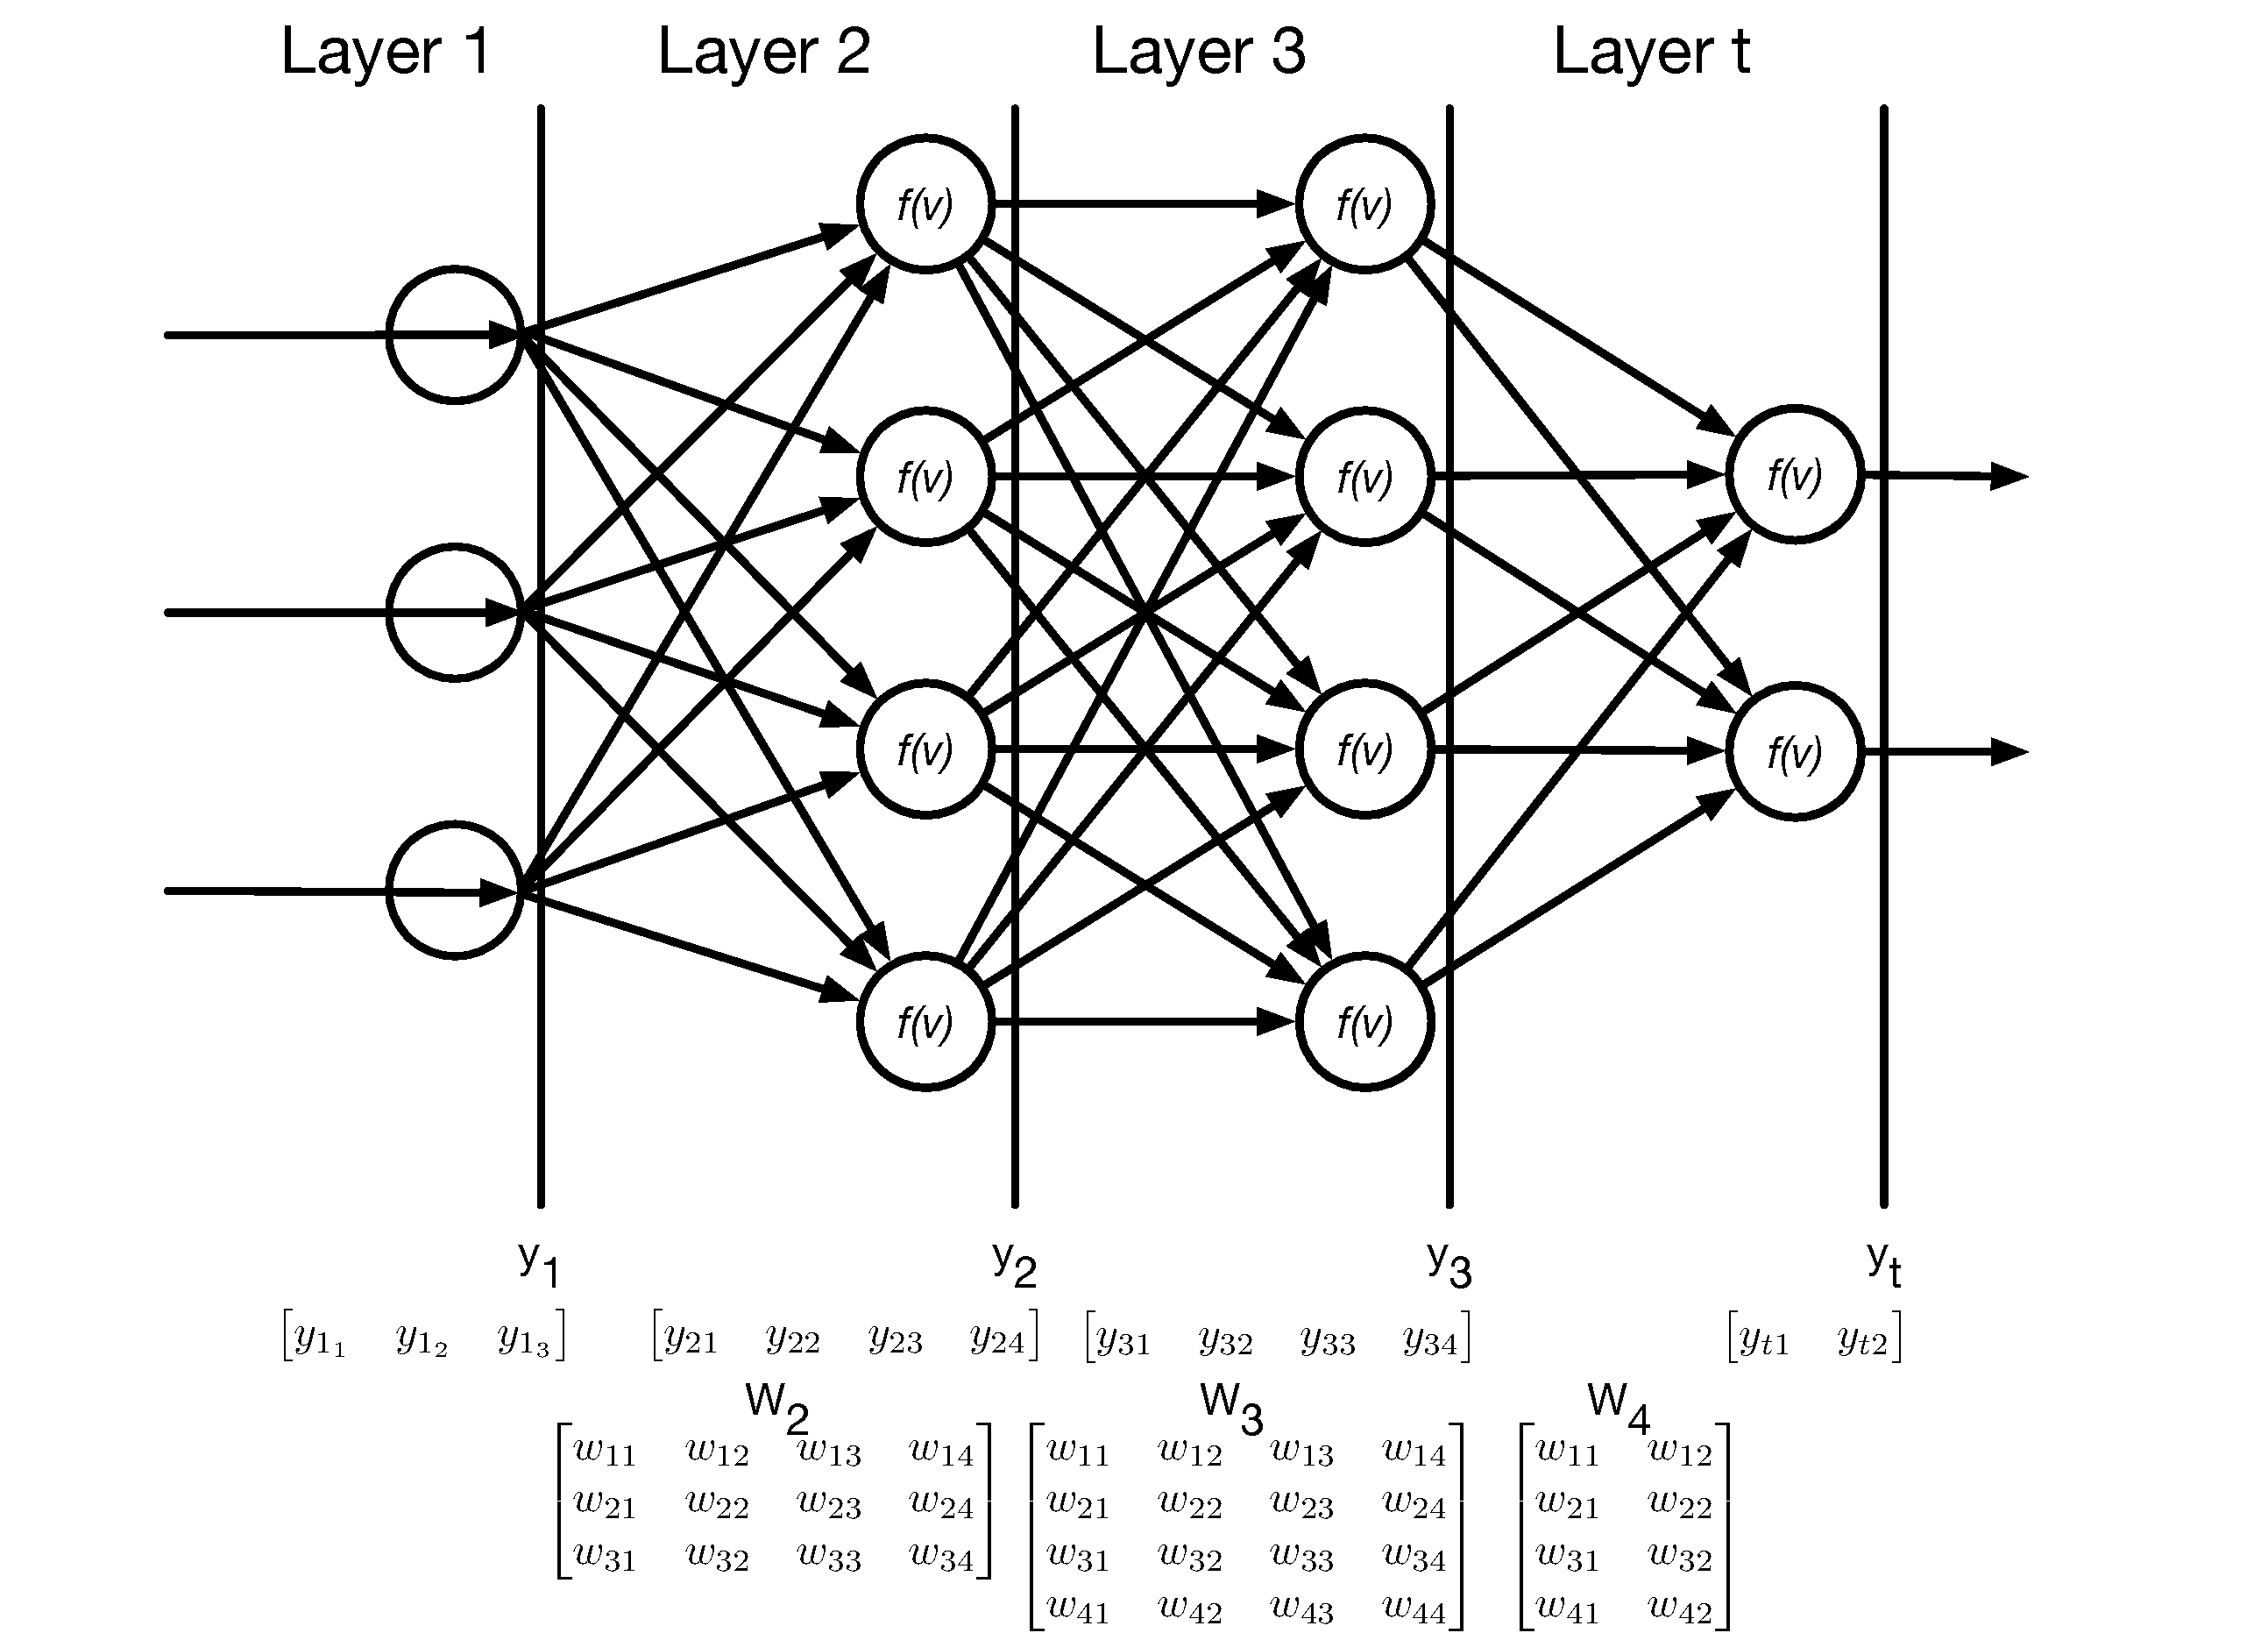
\includegraphics[width=.85\textwidth]{lectFF/nnEval.pdf}
\end{column}
\begin{column}{0.35\textwidth}
\begin{itemize}
\item $w_{i,j,k}$:
\item $i = $ layer
\item $j = $ input neuron
\item $k = $ output neuron
\end{itemize}
\end{column}
\end{columns}
\end{frame}
%***********************************************************
\begin{frame}[fragile]{GD for Deep NNs}

\begin{itemize}
	\item Just like all GD algorithms, it is iterative
	\begin{itemize}
	\item Assume loss function $L(W)$
	\item with learning rate, $\lambda$ 
	\item and where $W$ is a tensor of 2D weight matrices
	\item Then we have
	\end{itemize}
\end{itemize}

\begin{SQL}
$\textrm{Make a non-stupid guess for each } W_i$;
repeat {
  $W \leftarrow W - \lambda \nabla L (W)$;
} while (change in loss $> \epsilon$)
\end{SQL}
\end{frame}
%***********************************************************
\begin{frame}{Choosing a Loss Function}

\begin{itemize}
	\item There are many possible loss functions
	\item Let's assume one output neuron, one input data point; 
	\begin{itemize}
		\item Use $y_{i,k}$ to denote output from layer $i$, neuron $k$
		\item So in layer $t$ (``top'') just have $y_{t,1}$
		\item Hoped-for value is $y^{*}$
		\item Let's use squared loss: $L(W) = (y_{t,1} - y^{*})^2$
	\end{itemize}
	\item Extension to many data points, many outputs straightforward.                                                                          
\end{itemize}
\end{frame}
%***********************************************************
\begin{frame}{Our 1 I/O NN}

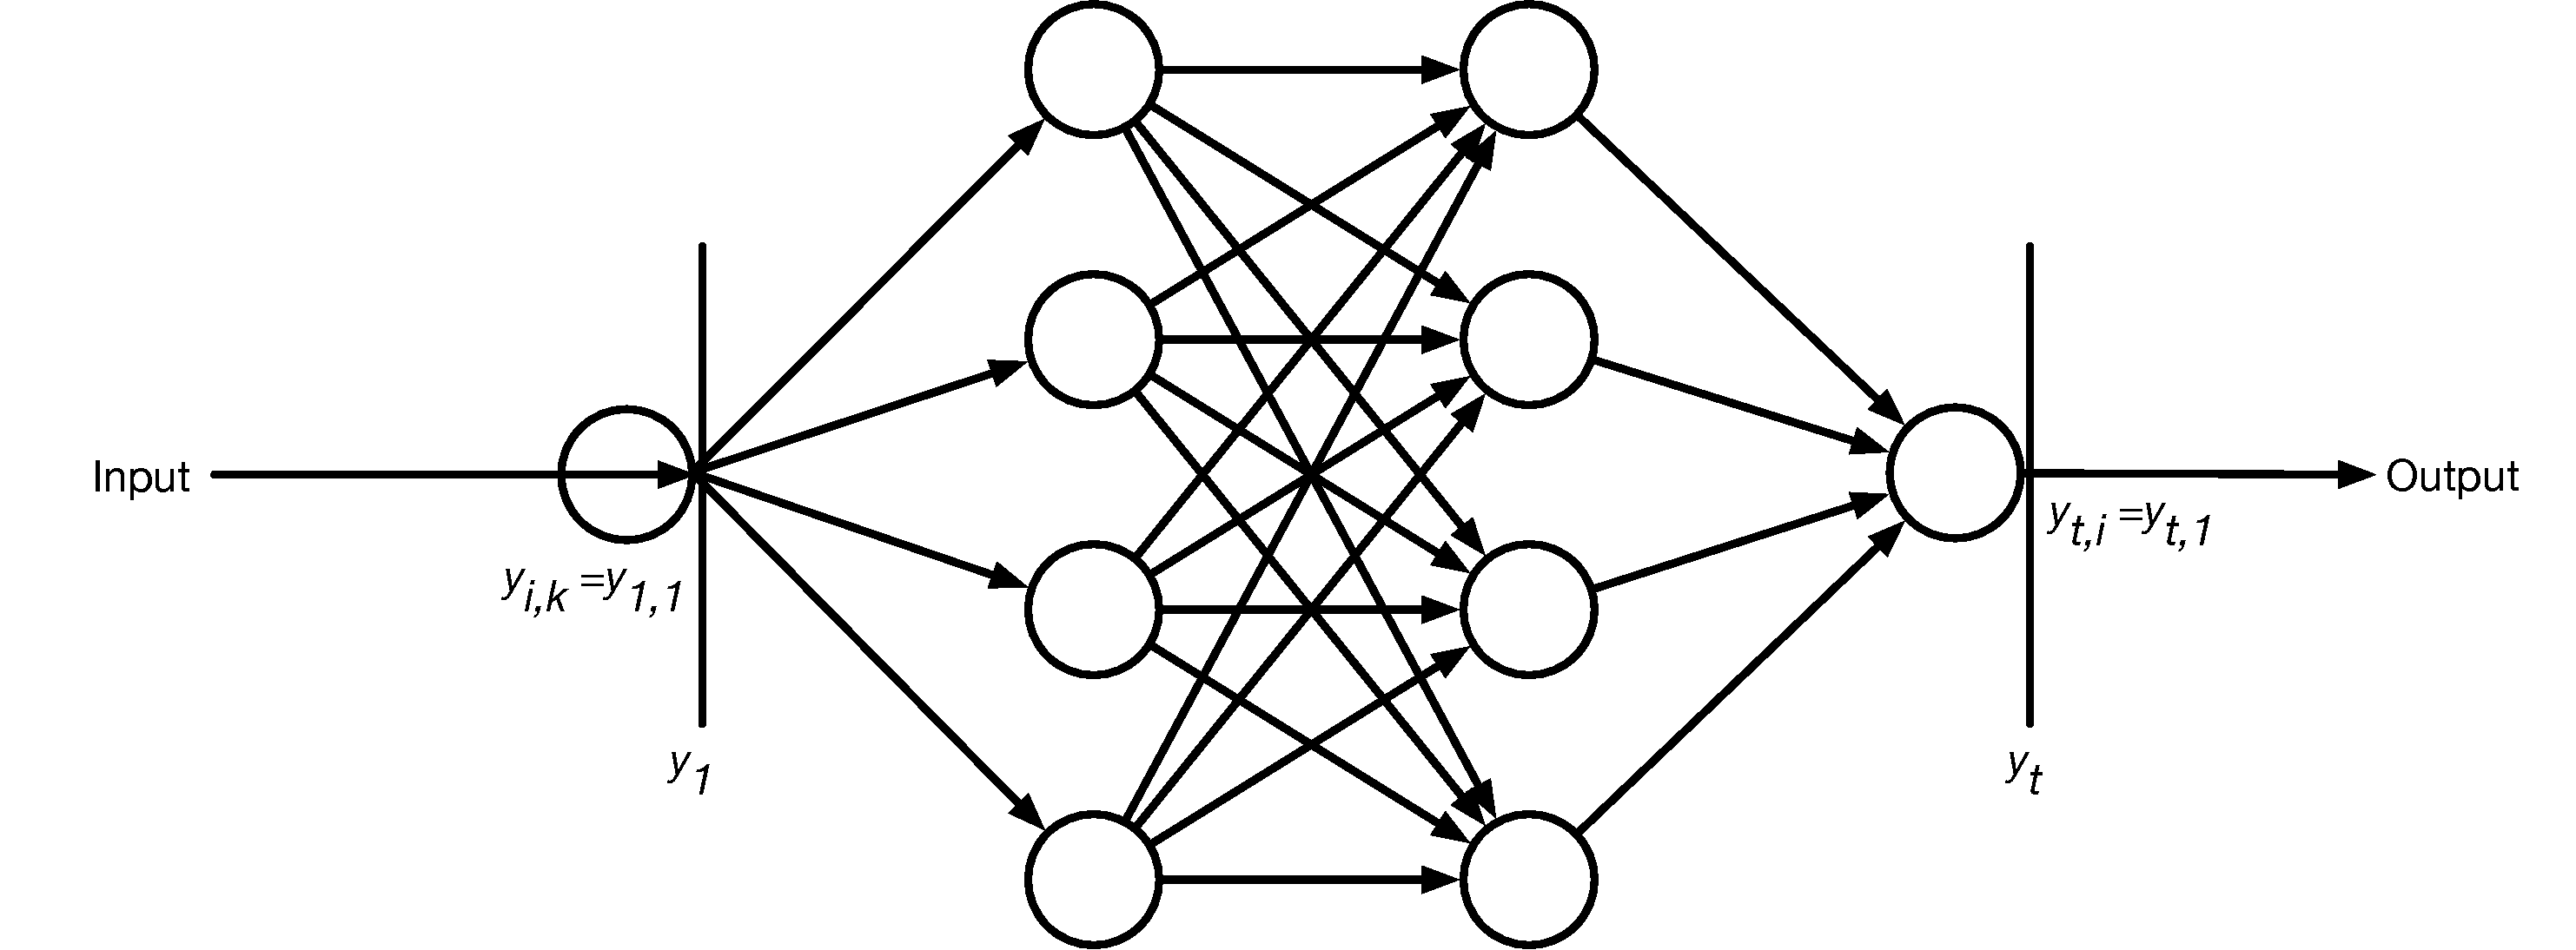
\includegraphics[width=1\textwidth]{lectBP/nnbp.pdf}
\end{frame}
%***********************************************************
\begin{frame}{Big Picture}

\begin{enumerate}
	\item Make a non-stupid guess for the weights
	\item Compute the value of the Loss function
	\item Redistribute the error from the Loss function among the weights 
\end{enumerate}
\begin{itemize}
	\item Weights that cause the error to increase will have larger activation values ($y$)
	\item And these will have larger values for $\frac{\partial L}{\partial W}$
\end{itemize}
% push back fraction of the error proportional to the weight
\end{frame}
%***********************************************************
\begin{frame}{Push Back Loss}

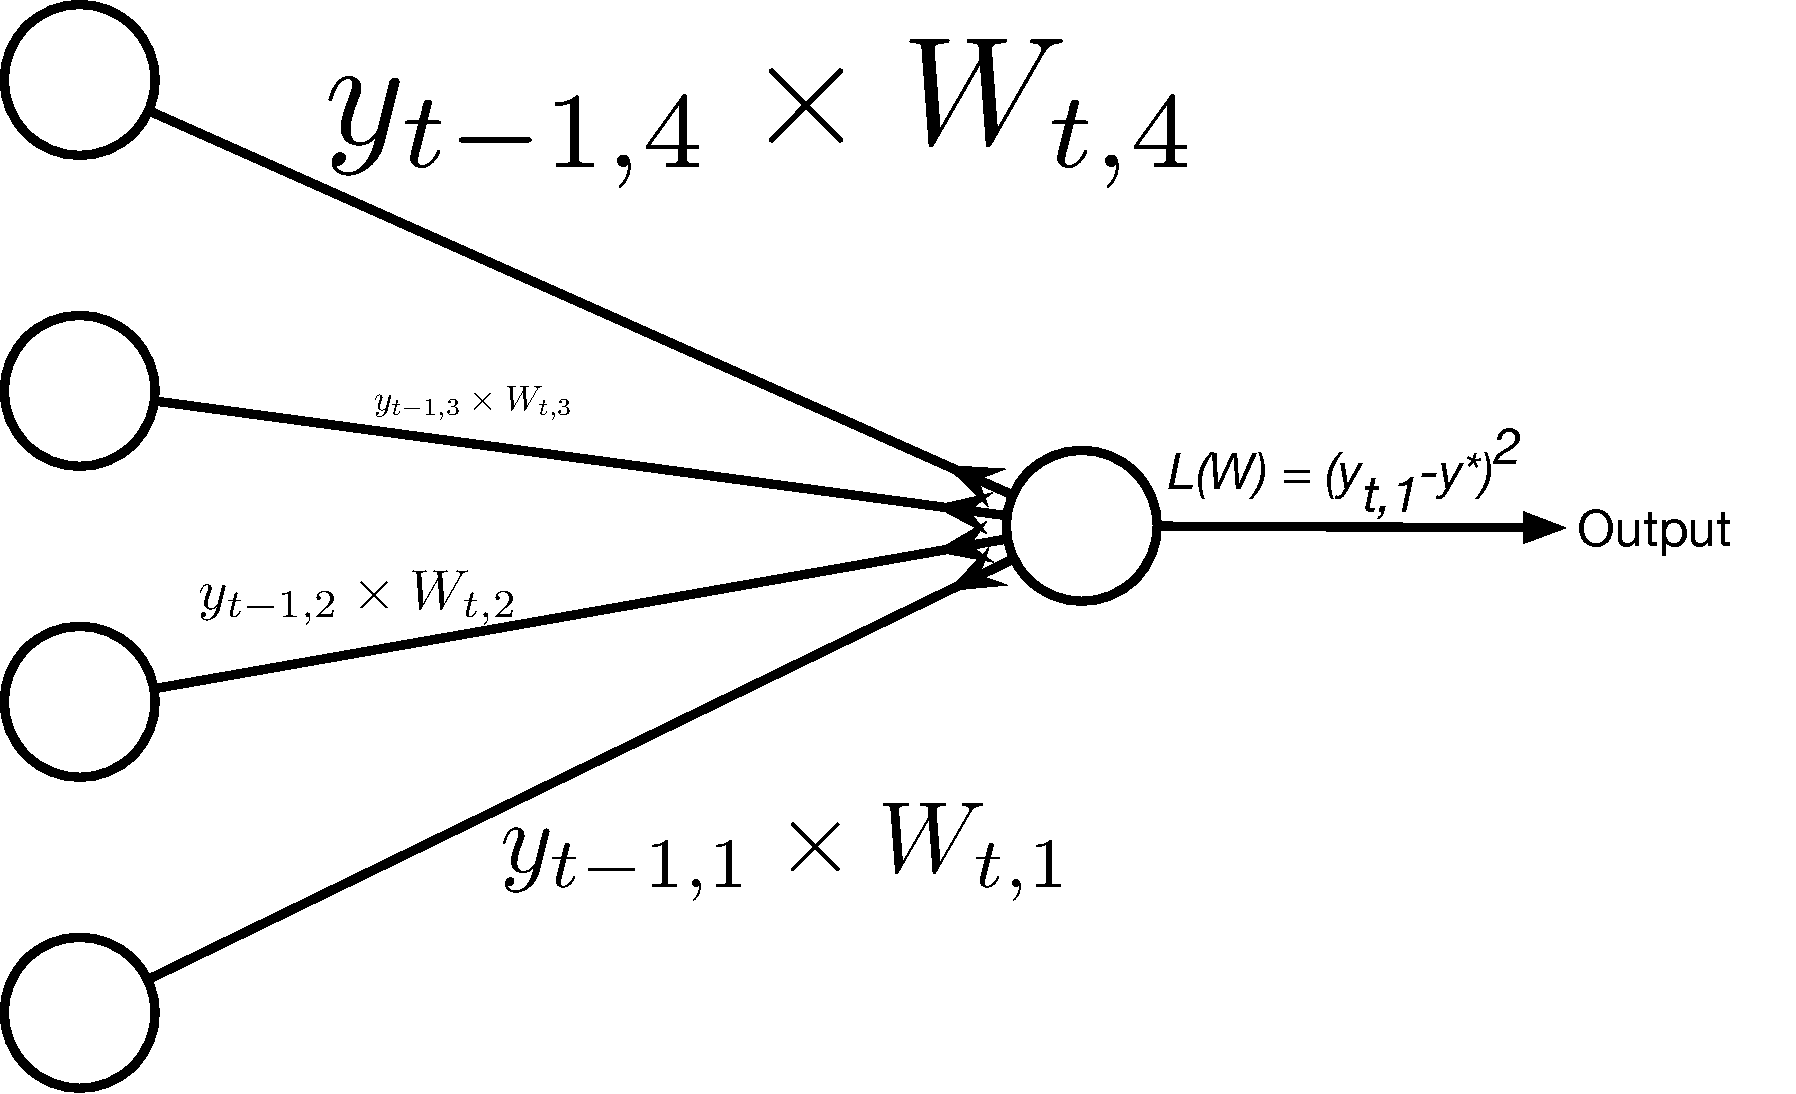
\includegraphics[width=.65\textwidth]{lectBP/pushBackLoss.pdf}
% kind of reminds me of PageRank
\end{frame}
%***********************************************************
\begin{frame}{From Inputs to Outputs to Weights}

\begin{itemize}
	\item Each input data point contributes to the cost and to the gradient
	\item Each ``pulls'' gradient descent in a certain direction
	\item Sum together the contribution to determine the overall direction of the gradient
	\item Move the weights that way
\end{itemize}
\end{frame}

%***********************************************************
\begin{frame}{Computing the Gradient}

\begin{itemize}
	\item Need to be able to differentiate $L$ wrt each weight
	\item Done by applying the chain rule:
	$$ \frac{\partial L}{\partial w_{i,j,k}} = \frac{\partial L}{\partial y_{i,k}} 
						\frac{\partial y_{i,k}}{\partial v_{i,k}}
						\frac{\partial v_{i,k}}{\partial w_{i,j,k}}$$
	\item $v_{i,k}$ is the weighted sum of activations sent into layer $i$, neuron $k$
	\item $v_{i,k} = \sum_{j'} w_{i,j',k} y_{i-1,j'}$
\end{itemize}
\end{frame}
%***********************************************************
\begin{frame}{Computing the Neuron Input}

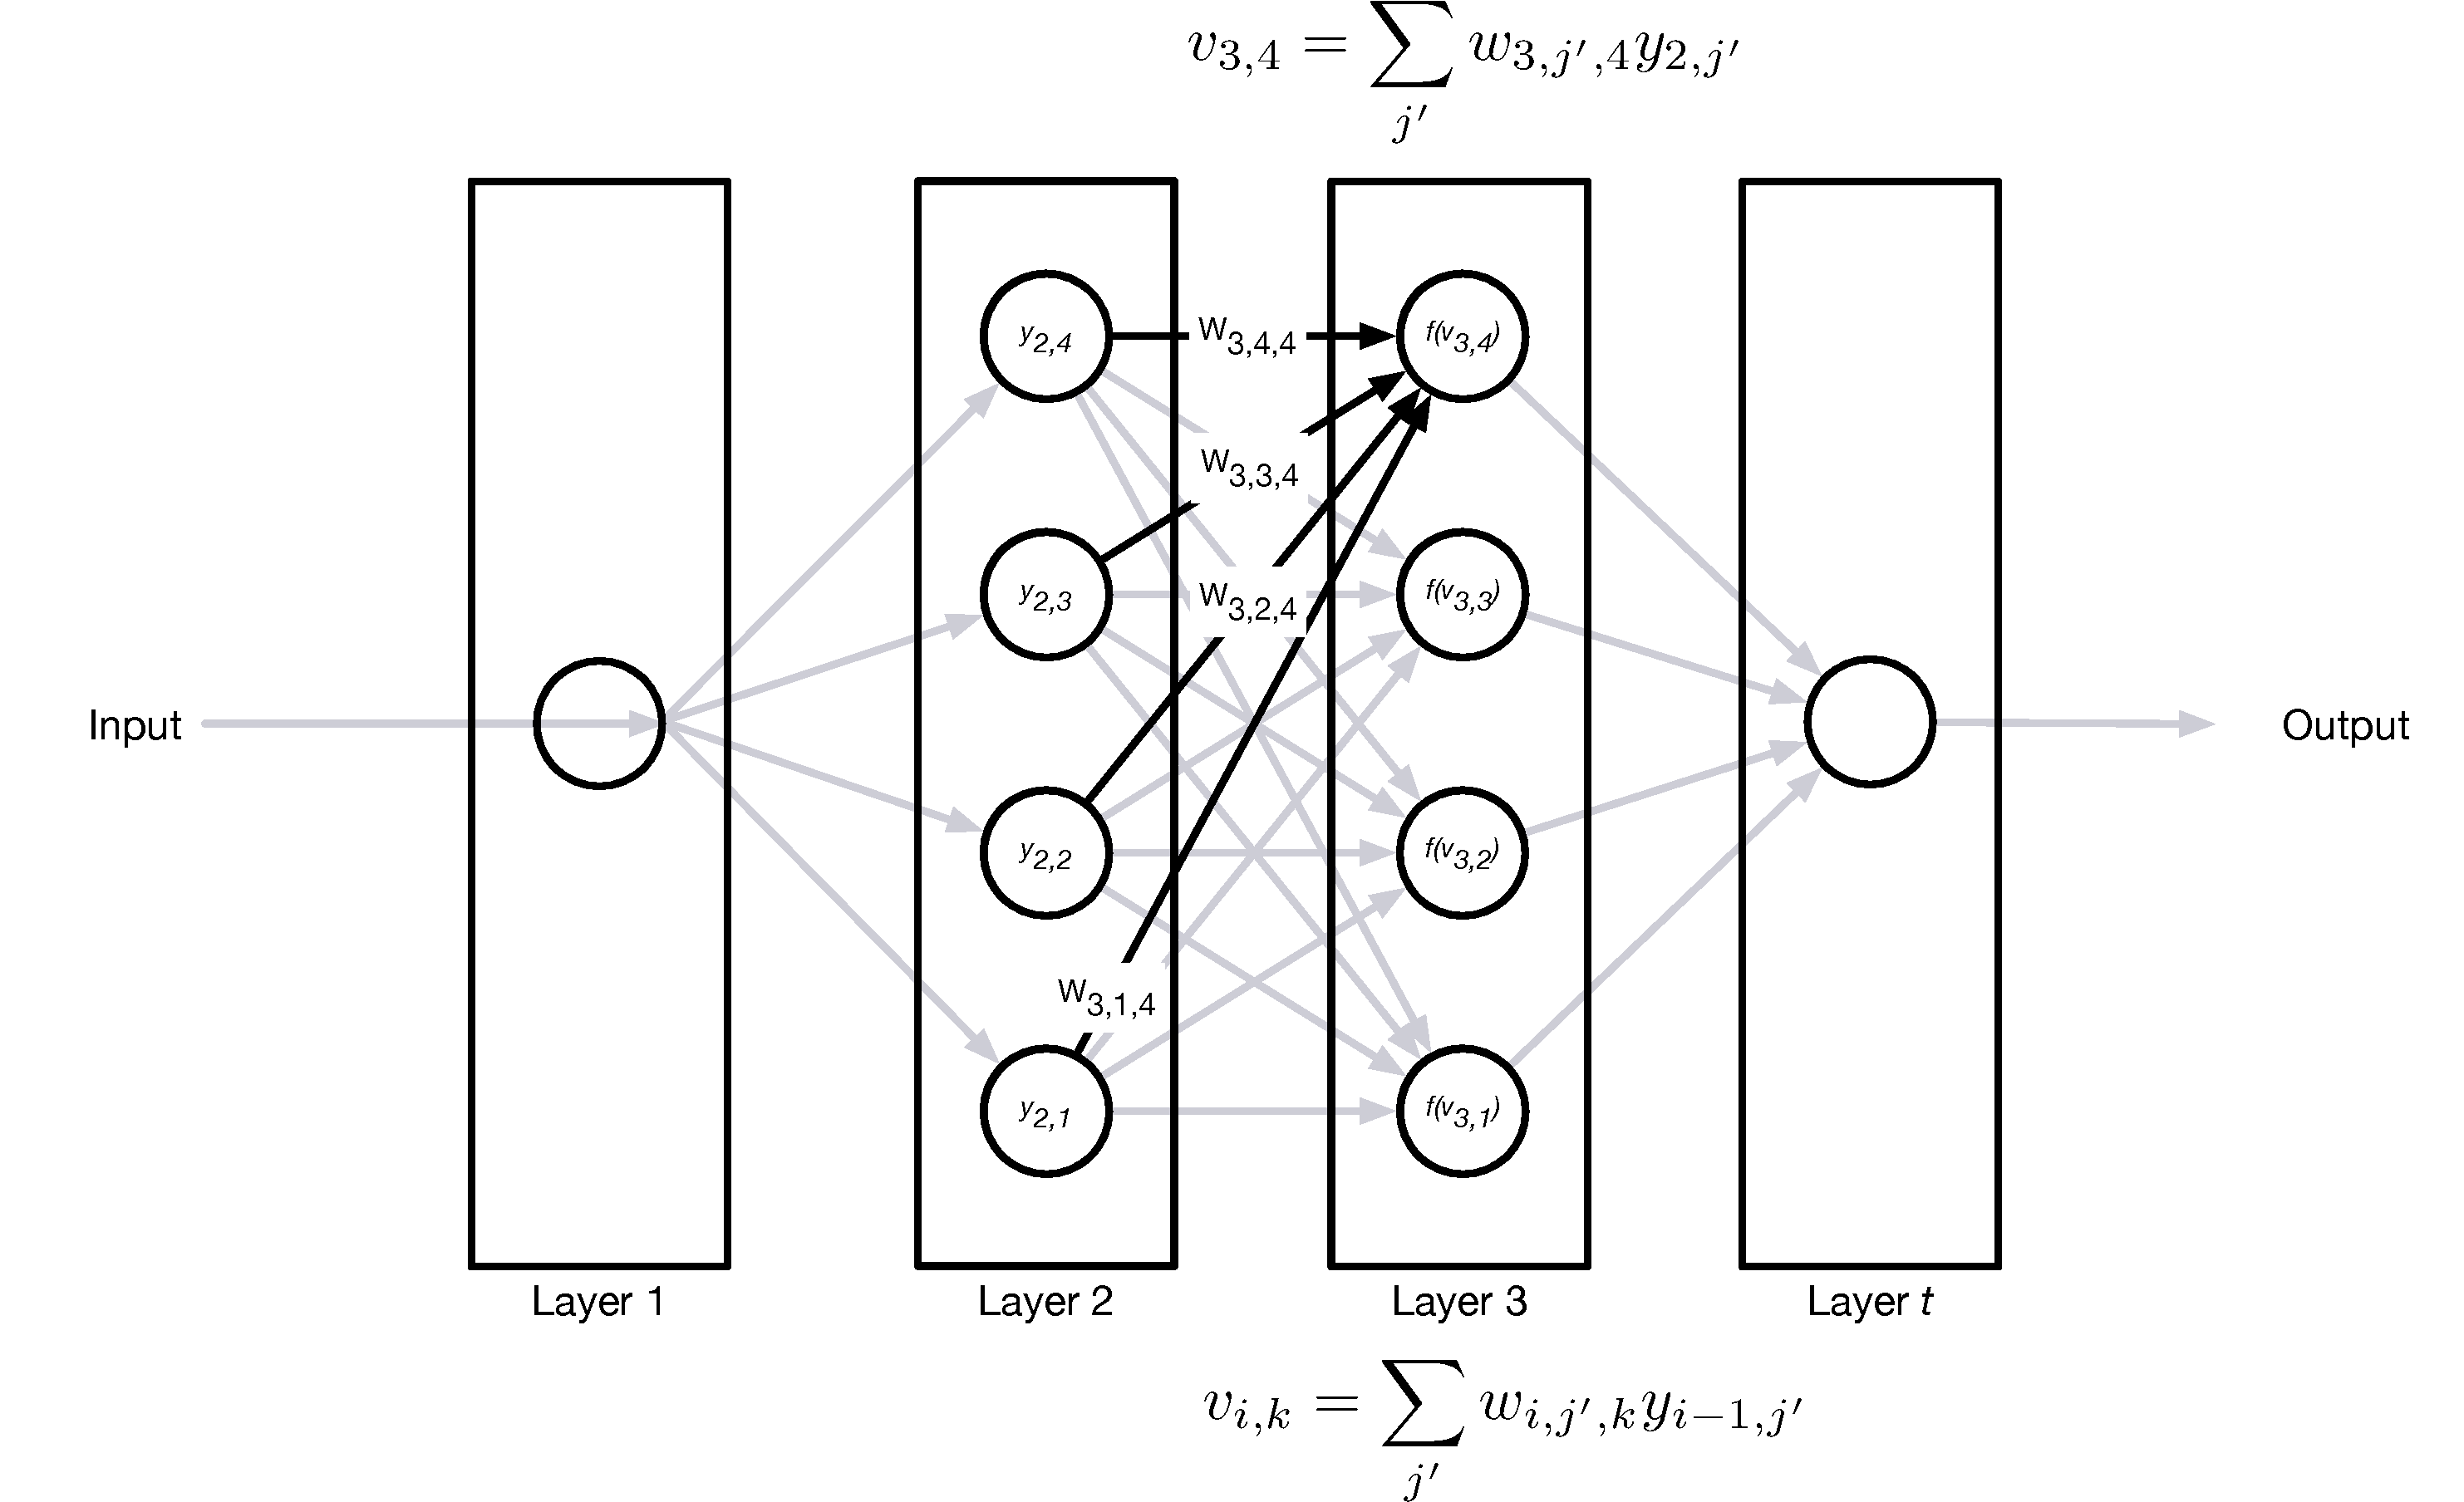
\includegraphics[width=0.75\textwidth]{lectBP/nnbpComputeG.pdf}
\end{frame}
%***********************************************************
\begin{frame}{Computing the Gradient}

\begin{itemize}
	\item Need to be able to differentiate $L$ wrt each weight
	\item Done by applying the chain rule:
	$$ \frac{\partial L}{\partial w_{i,j,k}} = \frac{\partial L}{\partial y_{i,k}} 
						\frac{\partial y_{i,k}}{\partial v_{i,k}}
						\frac{\partial v_{i,k}}{\partial w_{i,j,k}}$$
	$$ = \frac{\text{Loss}}{\text{Neuron Output}}\frac{\text{Neuron Output}}{\text{Neuron input}}\frac{\text{Neuron Input}}{\text{Weights}}$$
	\item Application of chain rule comes from chain of dependencies: 
	\begin{itemize}
		\item neuron output $y_{i,k}$ used to compute the loss
		\item neuron input $v_{i,k}$ used to compute neuron output $y_{i,k}$
		\item weight $w_{i,j,k}$ used to compute neuron input $v_{i,k}$
	\end{itemize}
	\item Note: No one actually does the math!
\end{itemize}
\end{frame}
%***********************************************************
%\begin{frame}[fragile]{GD for Deep NNs}
%
%\begin{SQL}
%$\textrm{Make a non-stupid guess for each } W_i$;
%repeat {
%  $W \leftarrow W - \lambda \nabla L (W)$;
%} while (change in loss $> \epsilon$)
%\end{SQL}
%\end{frame}
%***********************************************************
\begin{frame}{Now We Look At the Different Parts}

\begin{itemize} 
\item Explain
	$$ \frac{\partial L}{\partial w_{i,j,k}} = \frac{\partial L}{\partial y_{i,k}} 
						\frac{\partial y_{i,k}}{\partial v_{i,k}}
						\frac{\partial v_{i,k}}{\partial w_{i,j,k}}$$
	$$ \frac{\partial L}{\partial w_{i,j,k}} = 3 \times 1 \times 2 $$
\end{itemize}
\begin{enumerate} 
	\item Start with differentiating neuron output
	\item Then differentiating the neuron input
	\item And finally differentiating the loss
\end{enumerate}
\end{frame}
%***********************************************************
\begin{frame}{Differentiating Neuron Output}

\begin{itemize}
        \item We start with neuron output
	\item That is, $$\frac{\partial y_{i,j}}{\partial v_{i,j}}$$
\end{itemize}
\end{frame}
%***********************************************************
\begin{frame}{Computing the Gradient - Neuron Output}

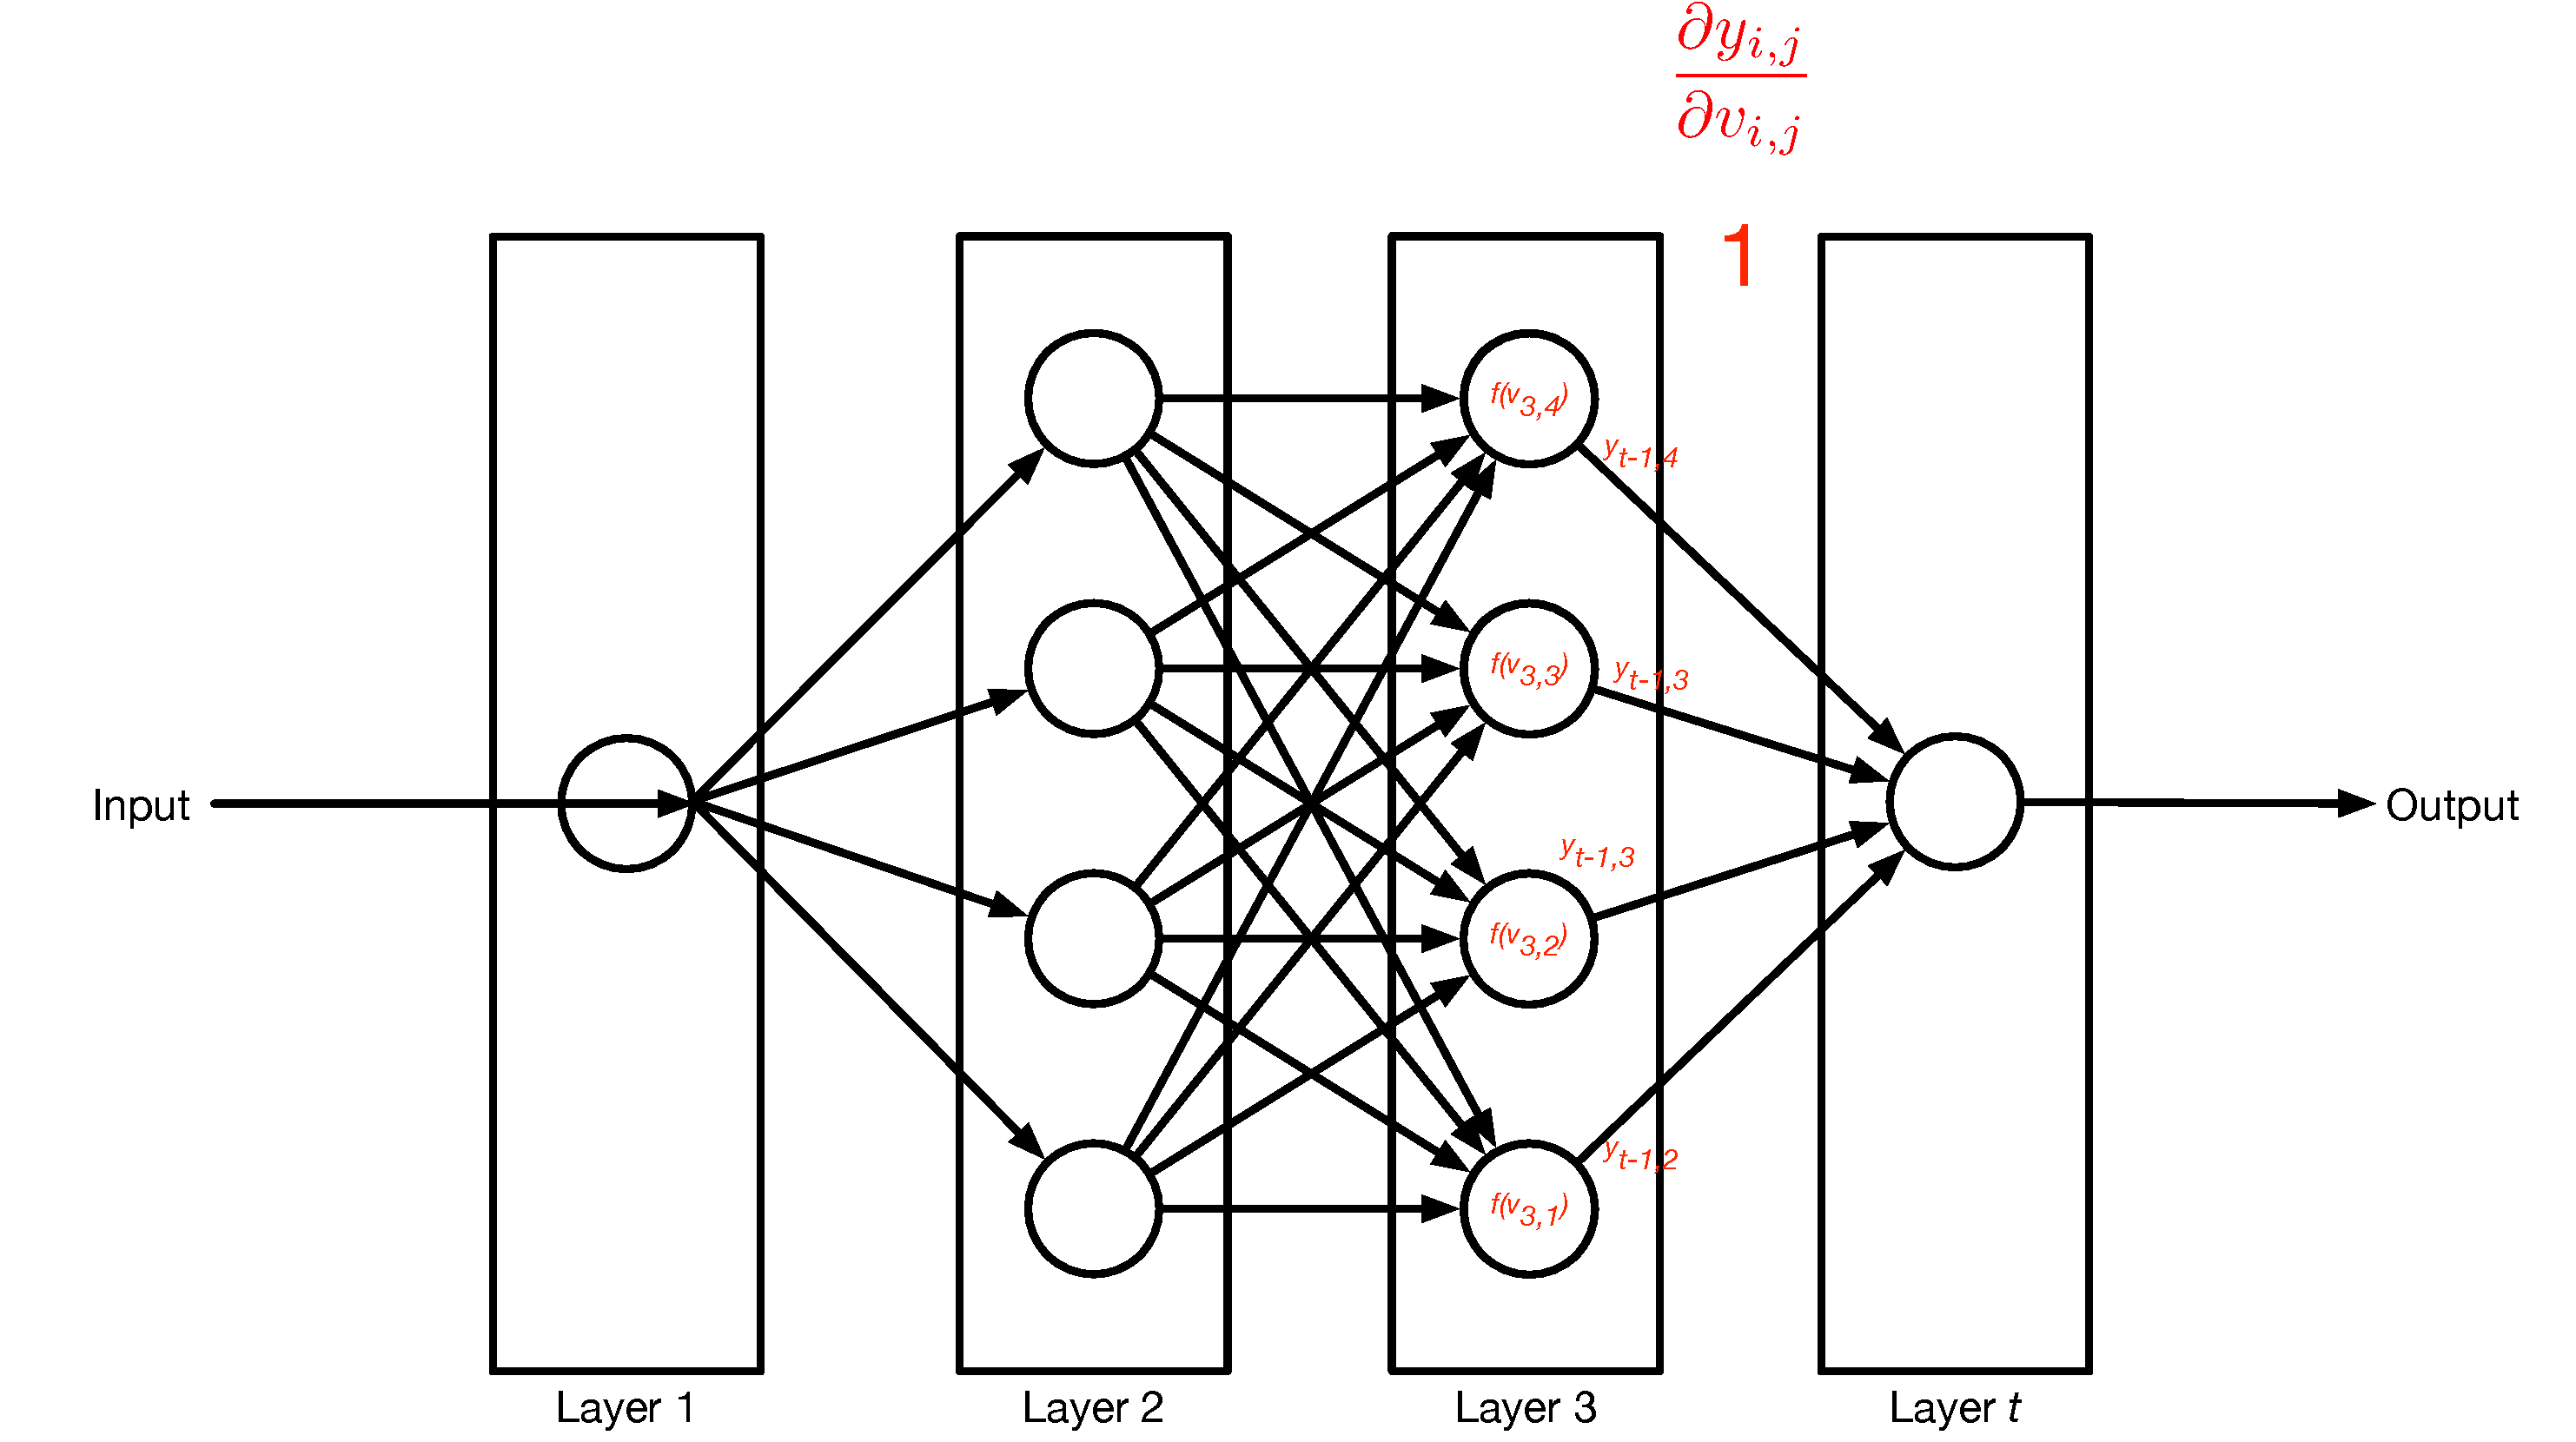
\includegraphics[width=1\textwidth]{lectBP/nnbpStep1.pdf}
\end{frame}
%***********************************************************
\begin{frame}{Differentiating Neuron Output}

\begin{itemize}
	\item Assume activation function is the logistic function
	$$f(v_{i,j}) = \frac{1}{1 + e^{-v_{i,j}}}$$
	\item Popular because result is magically simple
	\item Will skip algebra, but differentiating the logistic function gives us:
	$$\frac{df}{dv_{i,j}} = f(v_{i,j})(1 - f(v_{i,j}))$$
	\item So, since $y_{i,j} = f(v_{i,j})$,
	$$\frac{\partial y_{i,j}}{\partial v_{i,j}} = \frac{df}{dv_{i,j}} = 
		f(v_{i,j})(1 - f(v_{i,j}))$$
	\item Which is surprisingly nice for Logistic Regression
\end{itemize}

\end{frame}
%***********************************************************
\begin{frame}{Differentiating Neuron Input}

\begin{itemize} 
	\item Now time to deal with
	$$\frac{\partial v_{i,k}}{\partial w_{i,j,k}}$$
	\item Note that $v_{i,k}$ computes a dot product, so:x 
	$$\frac{\partial v_{i,k}}{\partial w_{i,j,k}} = \frac{\partial}{\partial w_{i,j,k}} 
		\sum_{j'} w_{i,j',k} y_{i-1,j'}$$
	\item This is just $y_{i-1,j}$, since all the $j'$s drop out, except for the case where $j'=j$
	\item We are summing over the prior layer's neurons
	\item Multiplying those outputs by the weights leading to the current layer
	\item For each neuron input, we only care about weights that go INTO this neuron
	\item Can ignore all the other weights in this layer
%	\item Note that if $i-1$ is the input layer, then $y_{i-1,j} = x_j$
%		\begin{itemize}
%		\item Where $x_j$ is the $j$th entry in the input vector
%		\end{itemize}
\end{itemize}
\end{frame}
%***********************************************************
\begin{frame}{Computing the Gradient - Neuron Input}

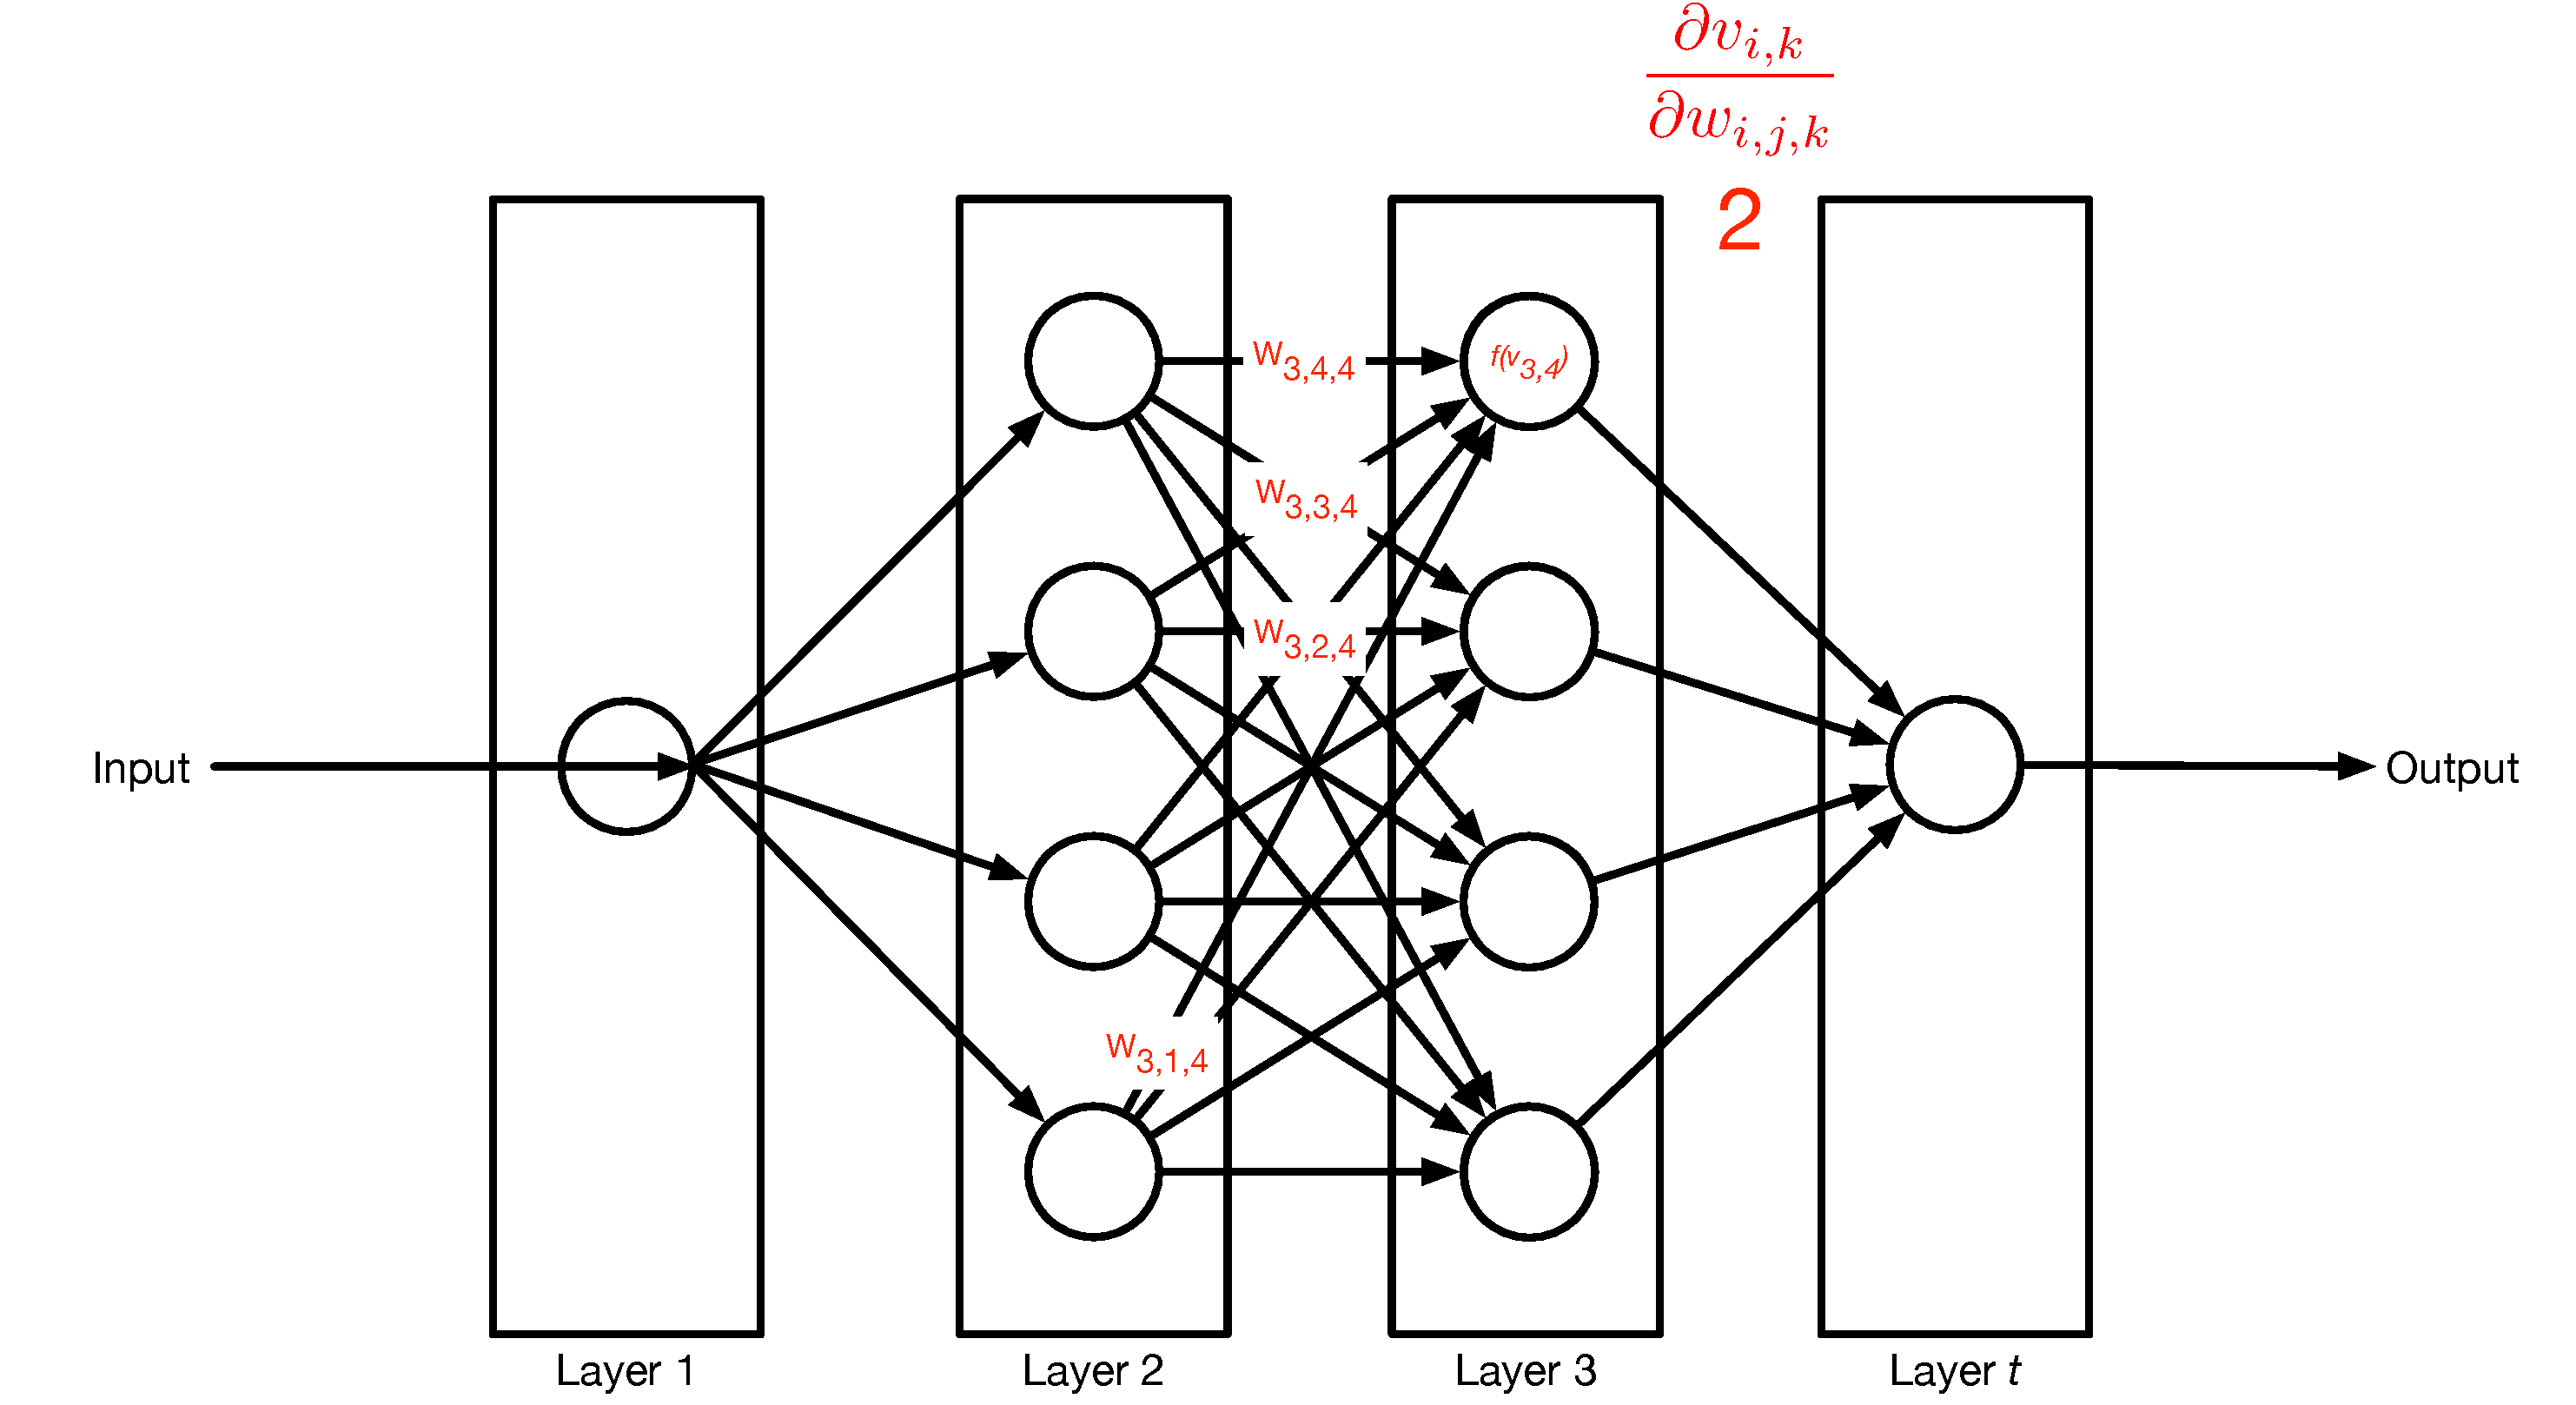
\includegraphics[width=1\textwidth]{lectBP/nnbpStep2.pdf}
\end{frame}
%***********************************************************
\begin{frame}{Differentiating Neuron Input from the Input Layer}

\begin{itemize} 
	\item Note that if $i-1$ is the input layer, then $y_{i-1,j} = x_j$
		\begin{itemize}
		\item Where $x_j$ is the $j$th entry in the input vector
		\end{itemize}
\end{itemize}
\end{frame}
%***********************************************************
\begin{frame}{Computing the Gradient - Neuron Input}

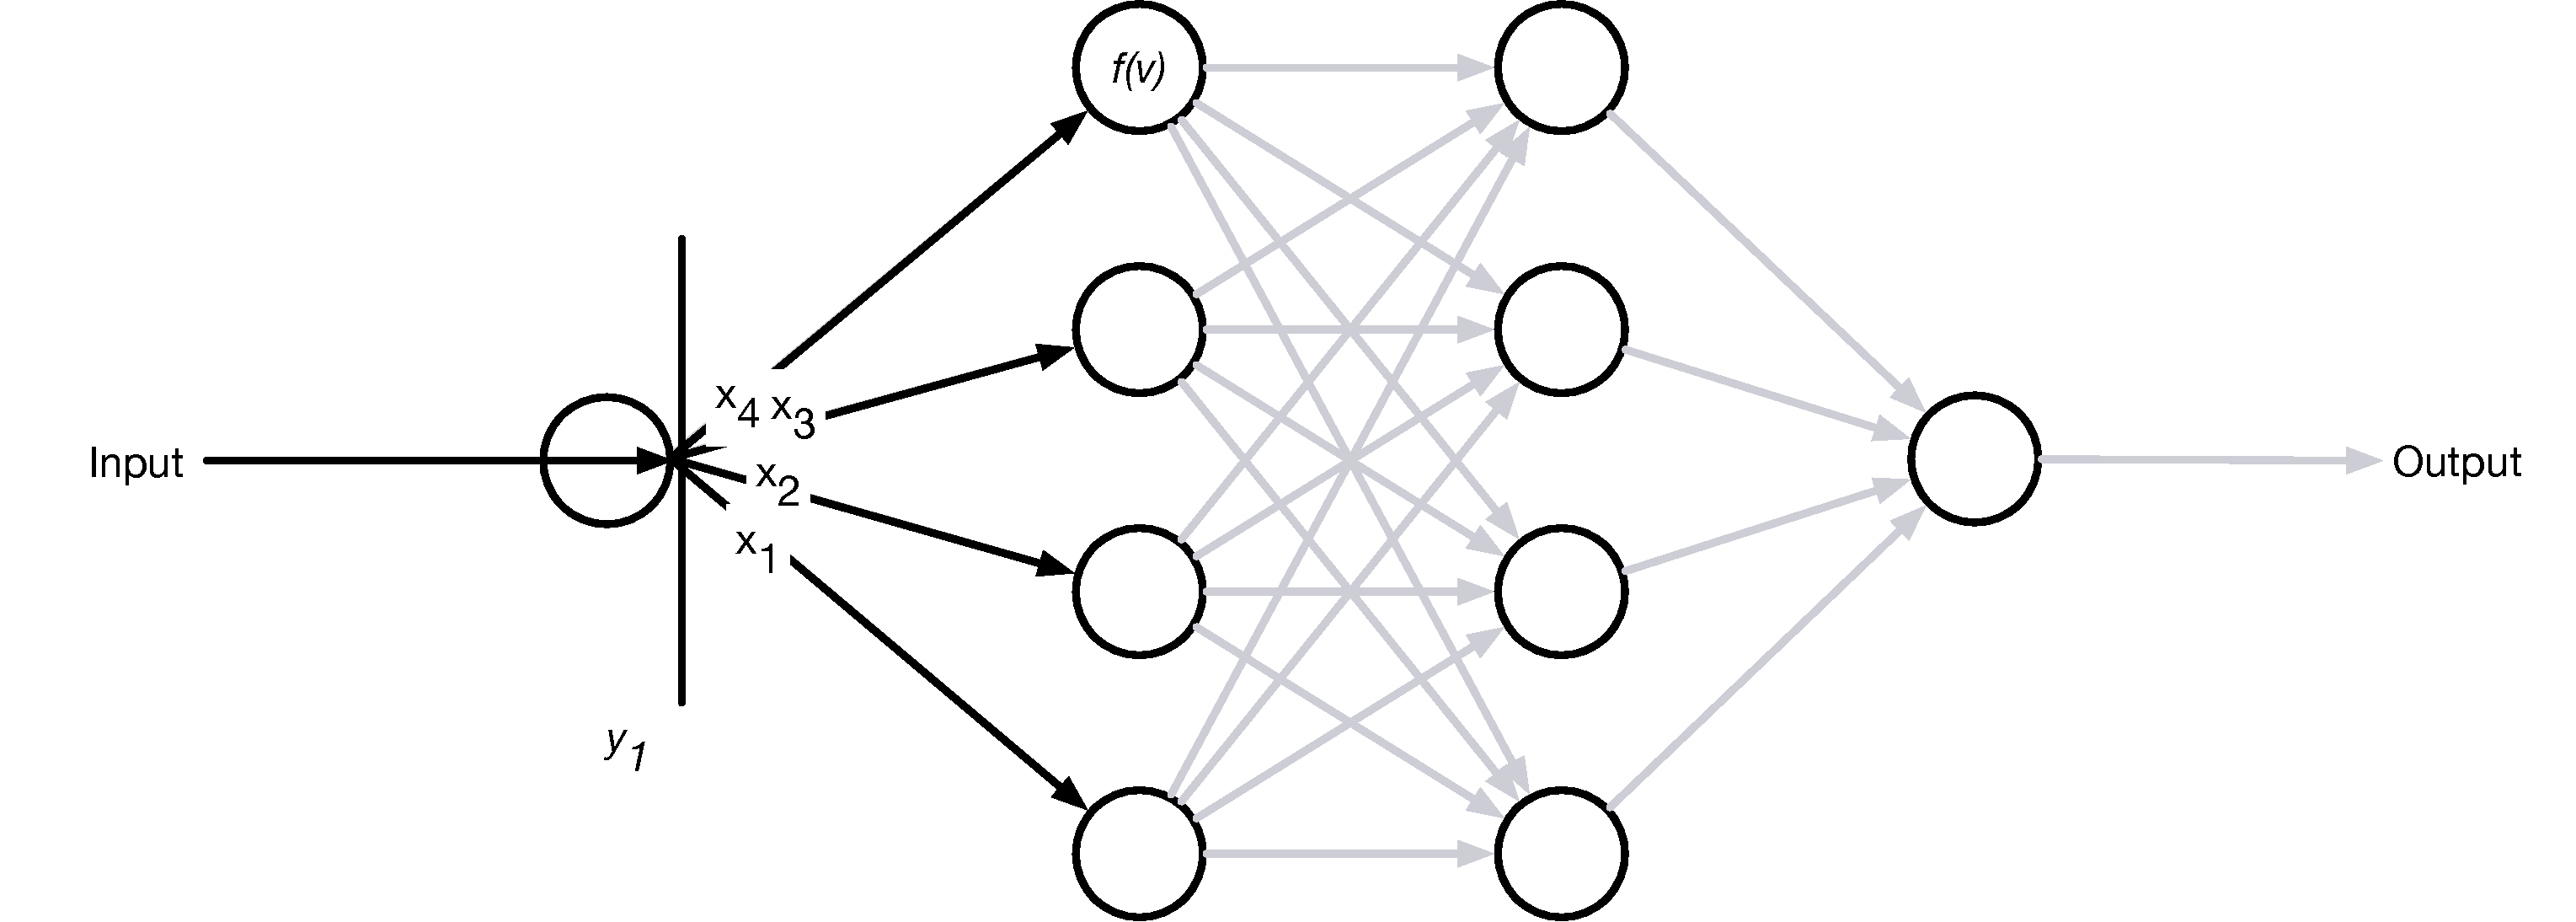
\includegraphics[width=1\textwidth]{lectBP/nnbpInput.pdf}
\end{frame}
%***********************************************************
\begin{frame}{Differentiating the Loss}

\begin{itemize}
	\item Next, need to be able to deal with differentiating the loss
		$$\frac{\partial L}{\partial y_{i,j}}$$
	\item If this is the output layer, it is easy:
	$$\frac{\partial L}{\partial y_{t,1}} = 2 (y_{t,1} - y^{*}) \approx (y_{t,1} - y^{*})$$
	\item Recall: $y^*$ is the hoped for output
	\item Can drop the $2$ since will be swallowed into the learning rate
\end{itemize}
\end{frame}
%***********************************************************
\begin{frame}{Computing the Gradient - Loss for Output Layer}

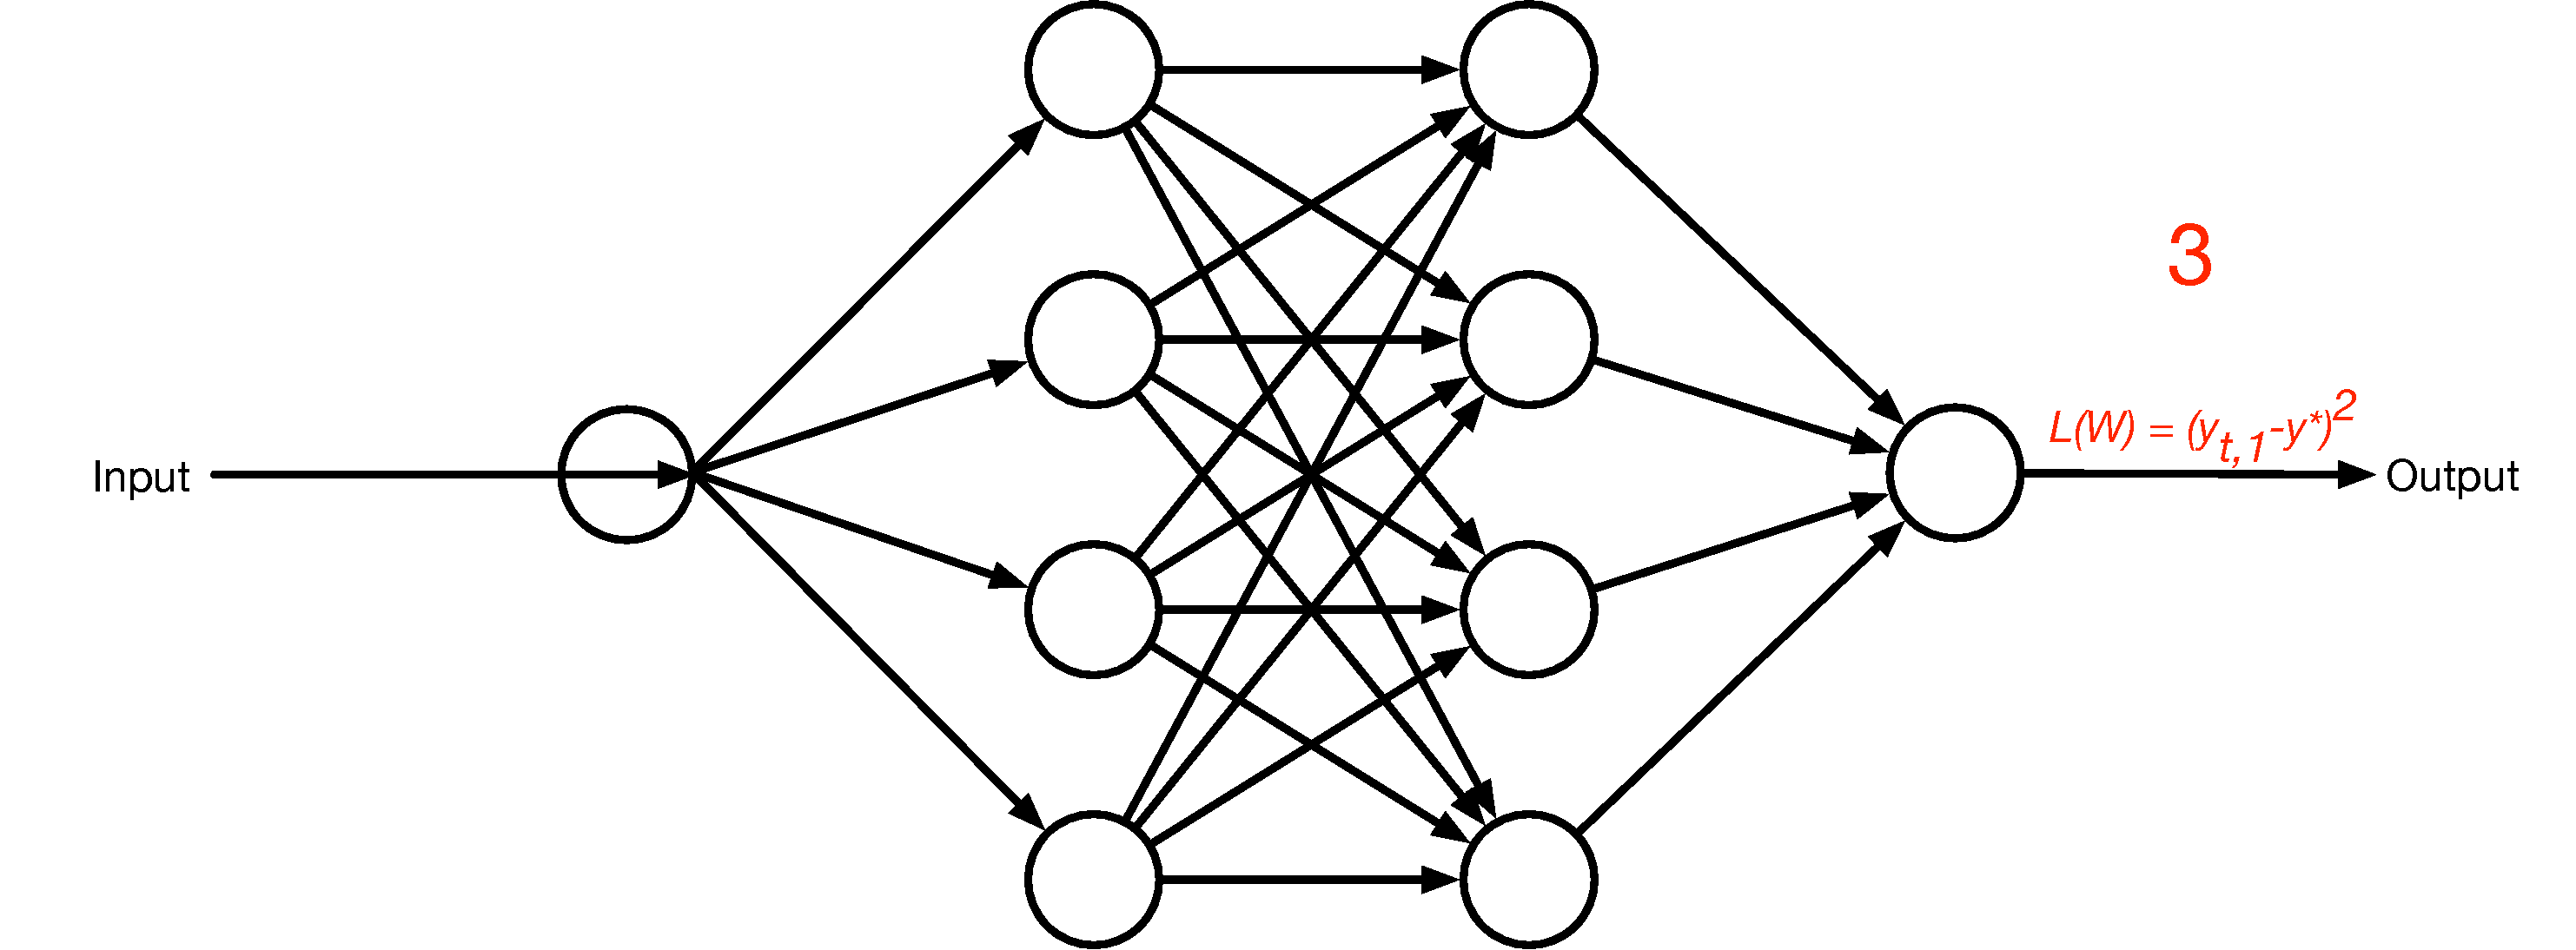
\includegraphics[width=1\textwidth]{lectBP/nnbpStep3.pdf}
\end{frame}
%***********************************************************
\begin{frame}{Differentiating the Loss}

\begin{itemize}
	\item Next, need to be able to deal with differentiating the loss
		$$\frac{\partial L}{\partial y_{i,j}}$$
	\item If this is the output layer, it is easy:
	$$\frac{\partial L}{\partial y_{t,1}} = 2 (y_{t,1} - y^{*}) \approx (y_{t,1} - y^{*})$$
	\item Recall: $y^*$ is the hoped for output
	\item Can drop the $2$ since will be swallowed into the learning rate
	\item[?] But what about the other layers?
\end{itemize}
\end{frame}
%***********************************************************
\begin{frame}{Sidebar: the Total Derivative}

\begin{itemize}
	\item Quick detour: idea of a ``total derivative'' (consequence of chain rule)
	\begin{itemize}
		\item Say we have a function $f$ of several variables $x_1, x_2, ...$
		\item Each of which is a function of variable $t$; we want $\frac{df}{dt}$
		\item Is computed via the ``total derivative'':
		$$\frac{df}{dt} = \frac{\partial f}{\partial x_1} \frac{\partial x_1}{\partial t} + 
			 \frac{\partial f}{\partial x_2} \frac{\partial x_2}{\partial t} + ...$$
	\end{itemize}
\end{itemize}
\end{frame}
%***********************************************************
\begin{frame}{Total Derivative Example}

\begin{itemize}
	\item A cylinder has radius and height of $2$ units 
	\begin{itemize}
		\item Recall $V = \pi r^2 h$
		\item It's getting bigger...
		\item Radius increases at 2 units/sec, height at 1 unit/sec
	\end{itemize}
\end{itemize}
\begin{center}
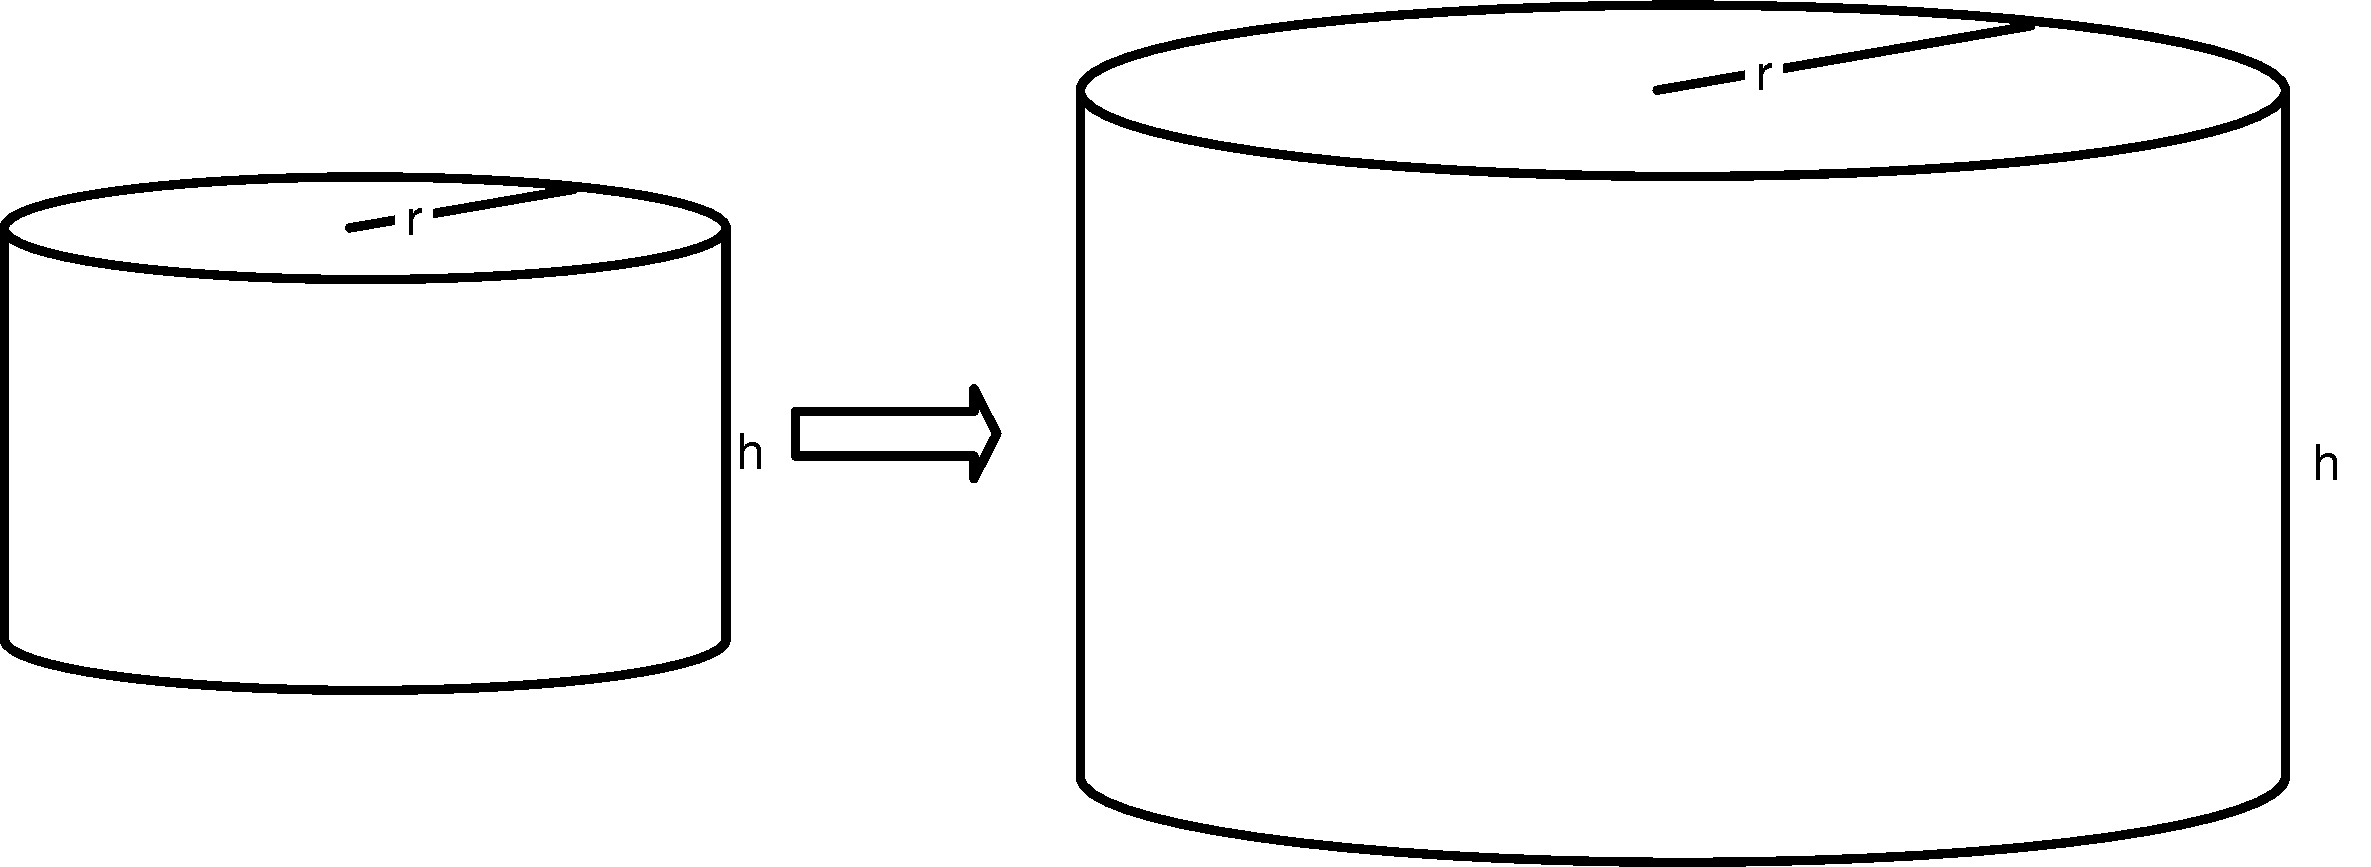
\includegraphics[width=.75\textwidth]{lectBP/cyl.pdf}
\end{center}
\end{frame}
%***********************************************************
\begin{frame}{Total Derivative Example}

\begin{itemize}
	\item A cylinder has radius, height of $2$ units 
	\begin{itemize}
		\item Recall $V = \pi r^2 h$
		\item It's getting bigger...
		\item Radius increases at 2 units/sec, height at 1 unit/sec
	\item What is the instantaneous rate of increase in volume?
		\begin{align}
		\frac{dV}{dt} &= \frac{\partial V}{\partial r} \frac{\partial r}{\partial t} +
                         \frac{\partial V}{\partial h} \frac{\partial h}{\partial t} \nonumber \\
			&= \pi 2r h \times  \Big( \frac{\partial r}{\partial t} \Big) + 
				\pi r^2 \times  \Big( \frac{\partial h}{\partial t} \Big) \nonumber \\
			&= \pi \times 2 \times 2  \times 2 \times (2) + \pi \times 2^2 \times (1) = 20\pi \textrm{ units}^3/\textrm{sec}\nonumber \end{align}
		\item Note: could substitute $r = 2 + 2t, h = 2 + t$ in $V = \pi r^2 h$
		\item Would get same answer
			using ``classic'' derivative over this new expression
	\end{itemize}
\end{itemize}
\end{frame}
%***********************************************************
\begin{frame}{Total Derivative vs. Partial Derivative}

\begin{itemize}
	\item Partial derivative: Other variables are treated as constants
	\item Total derivative: Other variables are NOT constant
\end{itemize}
\end{frame}
%***********************************************************
\begin{frame}{Differentiating Loss for Hidden Layers}

\begin{itemize} 
	\item Why is total derivative relevant?
	\begin{itemize}
	\item Note that Loss is a function of all the neuron inputs
	\item All $v$'s at layer $i+1$: $v_{i+1,1}, v_{i+1,2}, v_{i+1,3}, ...$
	\item Where $v_{i+1,k}$ is itself a function of $y_{i,j}$
	\item (Plus a lot of other things we'll treat as constants)
	\item This is exactly the case where $\frac{\partial L}{\partial y_{i,j}}$ must be computed using total
		derivative
	\item So take the total derivative wrt $y_{i,j}$:
		$$\frac{\partial L}{\partial y_{i,j}} = \sum_{k} \frac{\partial L}{\partial v_{i+1,k}}
			\frac{\partial  v_{i+1,k}}{\partial y_{i,j}}$$
	\item Partial of L wrt the $j$th neuron in layer $i$
	\item Recall that $y_{i,j}$ depends on all of the input weights
	\end{itemize}
\end{itemize}
\end{frame}
%***********************************************************
\begin{frame}{Computing the Gradient - Loss for Hidden Layers}

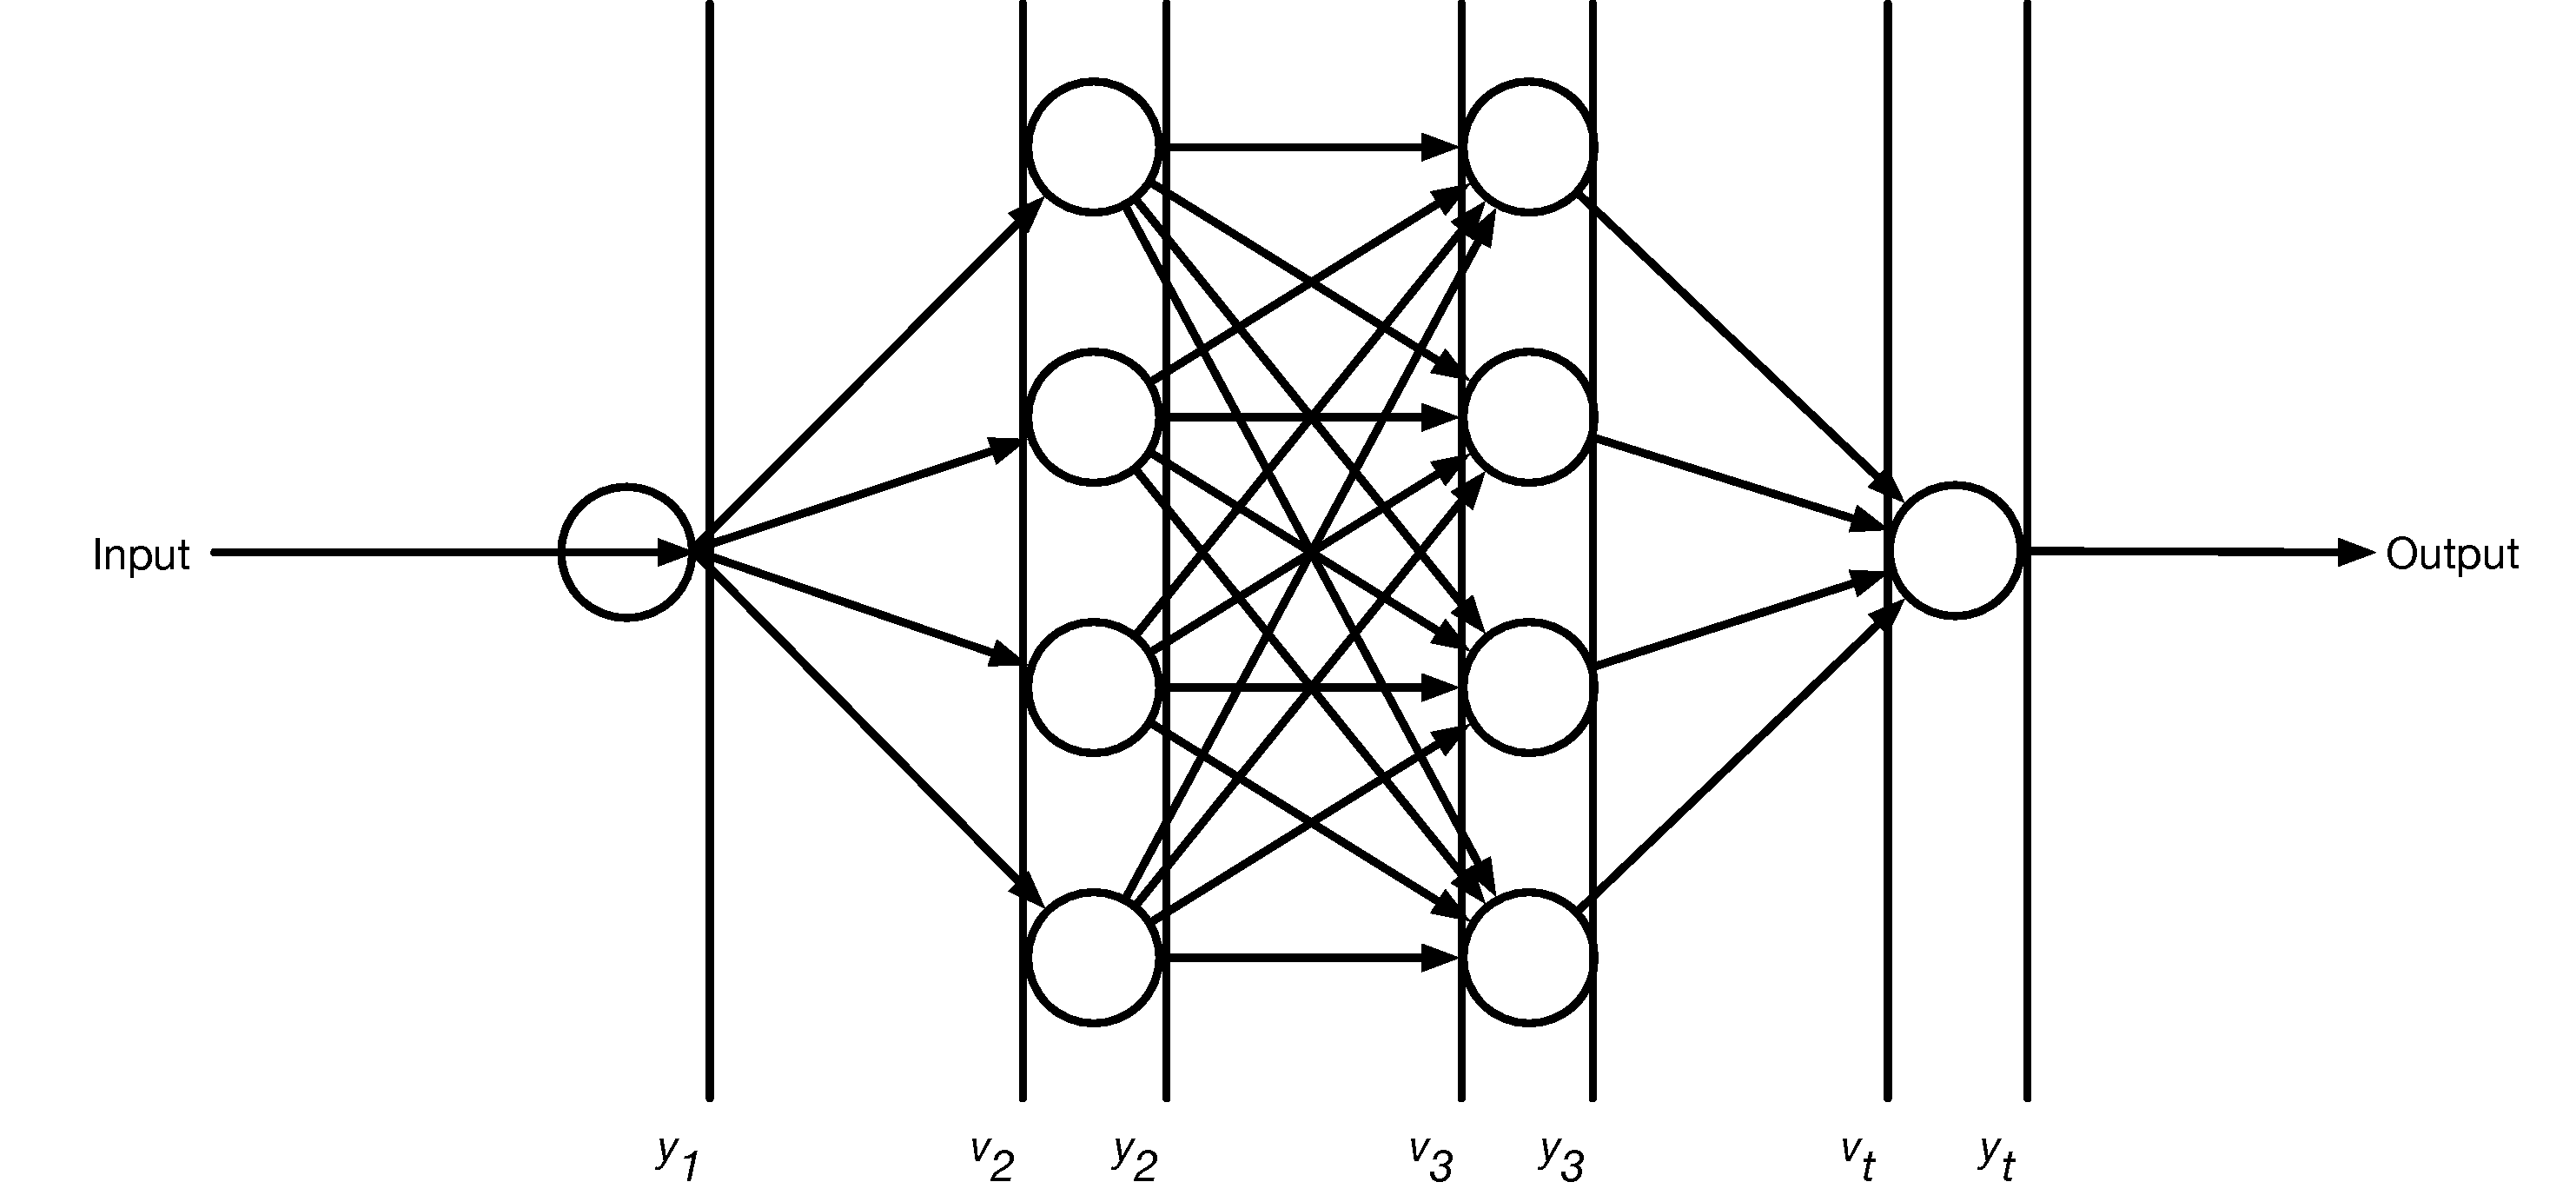
\includegraphics[width=1\textwidth]{lectBP/nnbpVs.pdf}
\end{frame}
%***********************************************************
\begin{frame}{Differentiating the Loss for Hidden Layers}
\begin{itemize}
	\item And since $\frac{\partial  v_{i+1,k}}{\partial y_{i,j}} = w_{i+1,j,k}$ 
%	\item That is, the change in inputs wrt prior outputs is the weight
	\item We have:
		$$\frac{\partial L}{\partial y_{i,j}} = \sum_{k} \frac{\partial L}{\partial v_{i+1,k}}
                        w_{i+1,j,k}$$
	\begin{itemize}
	\item Further, note that, by chain rule:
		 $$\frac{\partial L}{\partial v_{i+1,k}} = \frac{\partial L}{\partial y_{i+1,k}} 
                                                \frac{\partial y_{i+1,k}}{\partial v_{i+1,k}}$$
	\end{itemize}
	\item Refer to $\frac{\partial L}{\partial v_{i+1,k}}$ as $\delta_{i+1,k}$.
	\begin{itemize}
	\item So
		$$\frac{\partial L}{\partial y_{i,j}} = \sum_{k} \delta_{i+1,k}
                        w_{i+1,j,k}$$
	\end{itemize}
\end{itemize}
\end{frame}
%***********************************************************
\begin{frame}{Recursion!!}
\begin{itemize}
	\item Recall, 
	$$ \frac{\partial L}{\partial w_{i,j,k}} = \frac{\partial L}{\partial y_{i,k}} 
						\frac{\partial y_{i,k}}{\partial v_{i,k}}
						\frac{\partial v_{i,k}}{\partial w_{i,j,k}}$$
	\begin{itemize}
	\item And we can write this as:
	\begin{align} \frac{\partial L}{\partial w_{i,j,k}} &= 
		\left( \sum_{k'} \delta_{i+1,k'} w_{i+1,k,k'} \right)  
		\left( f(v_{i,k})(1 - f(v_{i,k})) \right)
			\left( y_{i-1,j} \right) \nonumber \\	
		&= \delta_{i,k} \left( y_{i-1,j} \right) \nonumber \end{align}
	\end{itemize}
	% NOTE: there are 3 different ways to represent the same equation
	% the middle one is key because we can store the values and use dynamic programming to calculate it more efficiently
	% we don't show a DP matrix because:
	%     it's transposed
	%.    not every layer has the same # of neurons
	%     if there were a matrix, it would grow from layer t to layer 1 (bottom to top)
\end{itemize}
\end{frame}
%***********************************************************
\begin{frame}{Breaking down the Transition}
\begin{center}
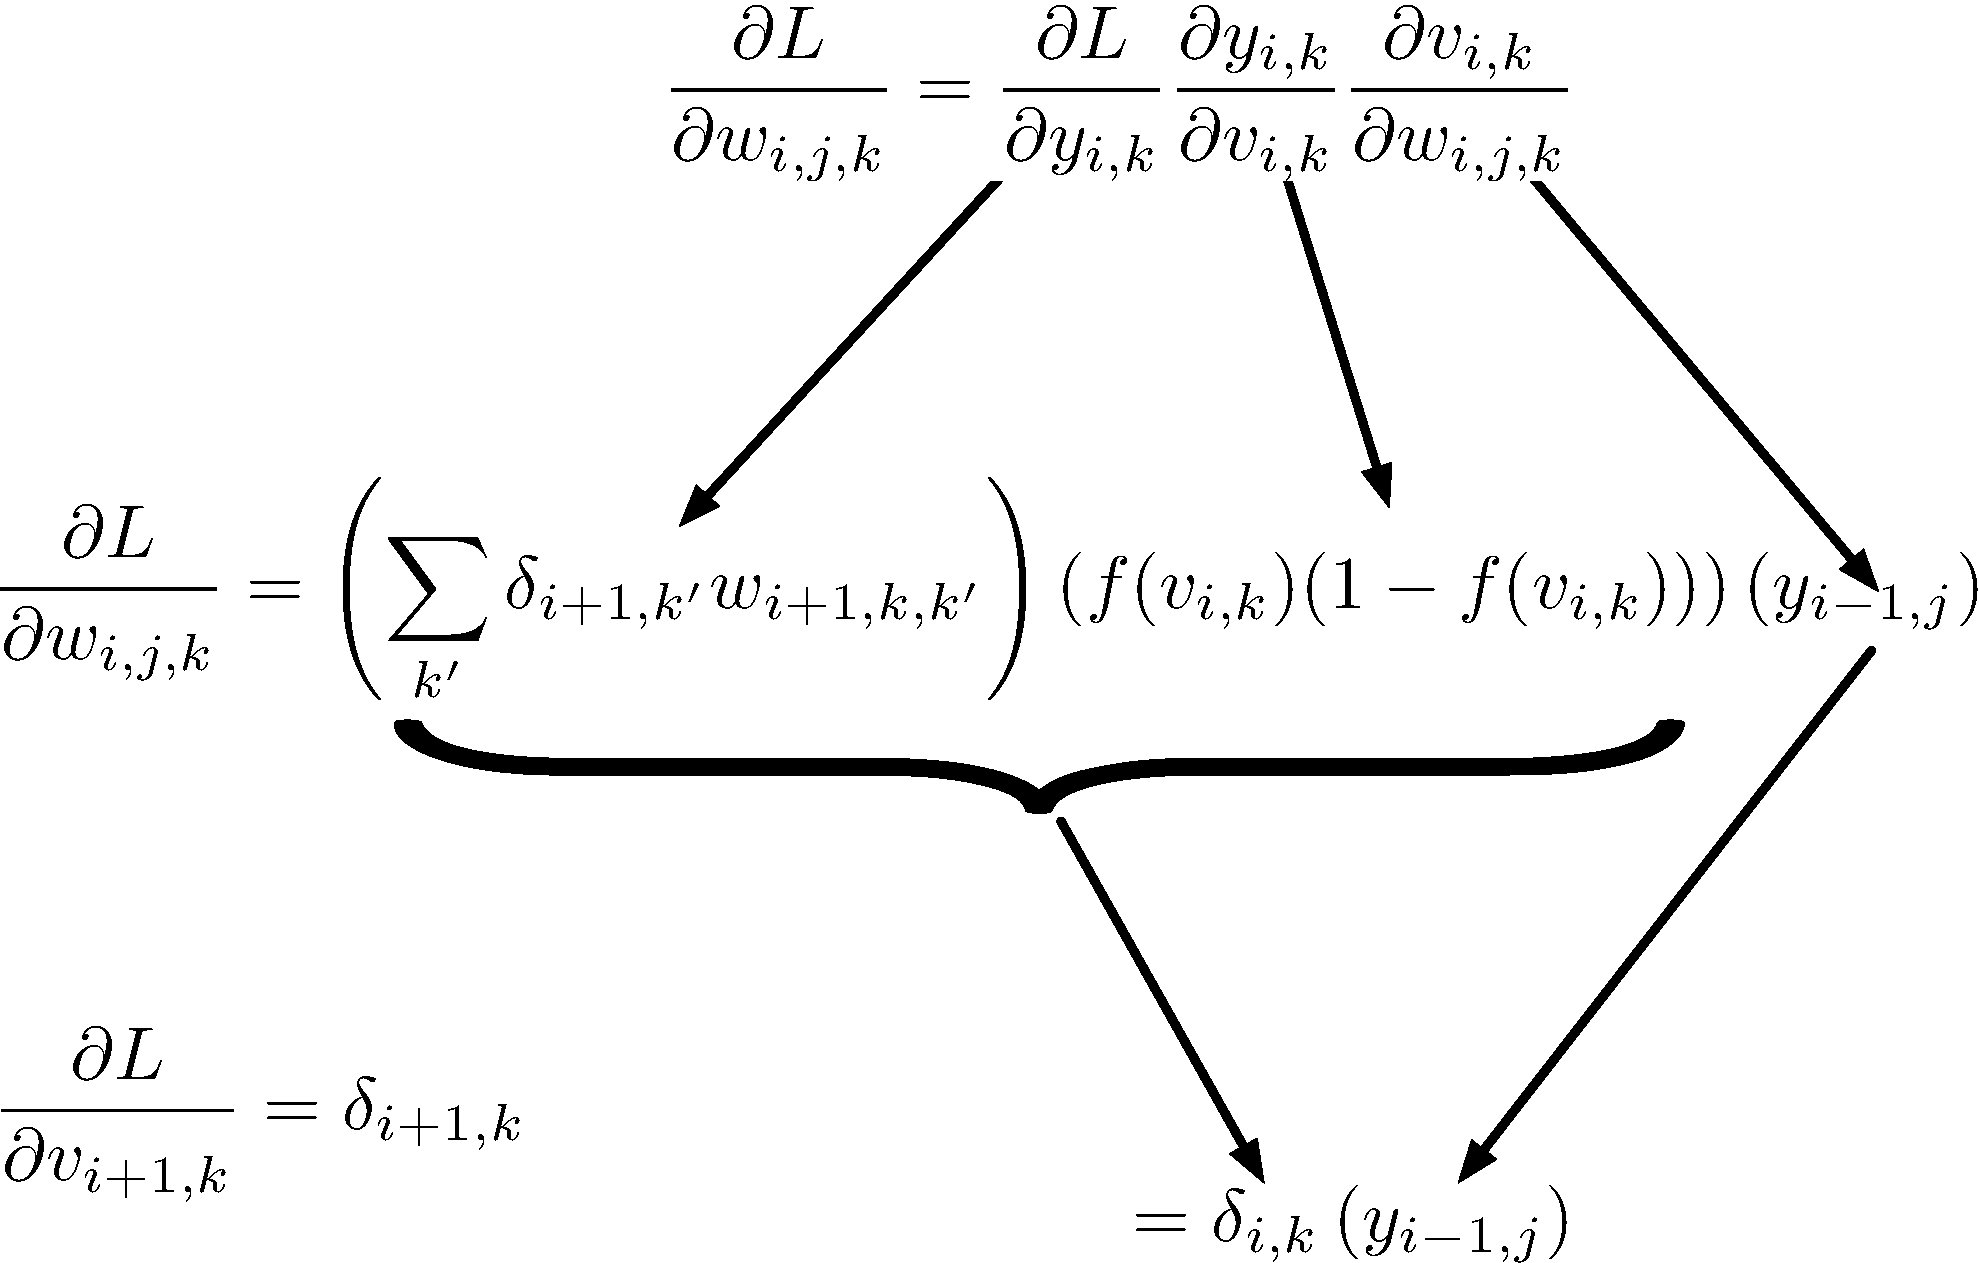
\includegraphics[width=.75\textwidth]{lectBP/delta.pdf}
\end{center}\end{frame}
%***********************************************************
\begin{frame}{Recursion!!}
\begin{itemize}
\item Remember our goal
	\item To be able to differentiate $L$ wrt each weight
	% NOTE: there are 3 different ways to represent the same equation
	% the middle one is key because we can store the values and use dynamic programming to calculate it more efficiently
	% we don't show a DP matrix because:
	%     it's transposed
	%.    not every layer has the same # of neurons
	%     if there were a matrix, it would grow from layer t to layer 1 (bottom to top)
	\item[]
	\begin{align} \frac{\partial L}{\partial w_{i,j,k}} &= 
		\left( \sum_{k'} \delta_{i+1,k'} w_{i+1,k,k'} \right)  
		\left( f(v_{i,k})(1 - f(v_{i,k})) \right)
			\left( y_{i-1,j} \right) \nonumber \\	
		&= \delta_{i,k} \left( y_{i-1,j} \right) \nonumber \end{align}
	\item This suggests a dynamic programming algorithm!
	\begin{itemize}
	\item Start at top, recurse back
	\item At layer $i$, to compute each $\frac{\partial L}{\partial w_{i,j,k}}$
		you use each $\delta_{i+1,k'}$ from previous layer
	\item As a side-effect of computing each $\frac{\partial L}{\partial w_{i,j,k}}$, you compute
		$\delta_{i,k}$
	\item Can record this and use when computing layer $i-1$ 
	\end{itemize}
\end{itemize}
\end{frame}

%***********************************************************
\begin{frame}{Dynamic Programming Algorithm}
\begin{itemize}
	\item First, make a forward pass thru the network
	\begin{itemize}
	\item Compute each $y_{i,k}$, $v_{i,k}$, $w_{i,j,k}$
	\item For each possible $i, j, k$
	\end{itemize}
	\item Then, make a backward pass thru the network, starting at the top layer
	\begin{itemize}
	\item Top layer is base case; compute $$\delta_{t,1} = \frac{\partial L}{\partial y_{t,1}}
                                                \frac{\partial y_{t,1}}{\partial v_{t,1}} =
			 f(v_{t,1})(1 - f(v_{t,1})) (y_{t,1} - y^{*})$$
	\item And then $$\frac{\partial L}{\partial w_{t,j,1}} = \delta_{t,1}
		 y_{t-1,j}$$
	\end{itemize}
\end{itemize}
\end{frame}
%***********************************************************
\begin{frame}{DP for Back-propagation: Other Layers}
\begin{itemize}
	\item Then at every other layer, want $\frac{\partial L}{\partial w_{i,j,k}}$, for each $j$, $k$ pair
	\item To do this:
	\begin{itemize}
	\item At layer $i$, for a given $j$, $k$ pair
	\item First compute $\delta_{i,k} =  \left( \sum_{k'} \delta_{i+1,k'} w_{i+1,k,k'} \right)
                \left( f(v_{i,k})(1 - f(v_{i,k})) \right)$; save this value
	\item Next compute $\frac{\partial L}{\partial w_{i,j,k}} = \delta_{i,k} y_{i-1,j}$
	\end{itemize}
	\item Keep recursing until you have each $\frac{\partial L}{\partial w_{2,j,k}}$
	\item All of the $\frac{\partial L}{\partial w_{i,j,k}}$ values together then constitute $\nabla L(W)$
	\item Use in an iteration of GD
\end{itemize}
\end{frame}
%***********************************************************

\begin{frame}{How To Implement Learning?}
\begin{itemize}
	\item This math has been known for many years
	\item Once you understand it, is quite simple
	\item So would be easy to implement learning directly in Python
	\item But applies to particular narrow case:
		\begin{itemize}
		\item Fully-connected network
		\item Logistic activation
		\item Feed-forward
		\item L2 loss
		\item One output neuron
		\item One data item
		\end{itemize}
\end{itemize}
\end{frame}
%***********************************************************

\begin{frame}{What If Your Network Is Different?}

\begin{itemize}
	\item Some changes are easy:
	\begin{itemize}
		\item Different loss: only changes $\frac{\partial L}{\partial y_{t,1}}$
		\item Multiple data points in a batch: 
			compute $\frac{\partial L}{\partial w_{i,j,k}}$ wrt each, and
			then add them up (can be made efficient with vector/matrix ops)
		\item Different activation: only changes $\frac{\partial y_{i,j}}{\partial v_{i,j}}$
	\end{itemize}
	\item But some are hard...
	\item What about adding convolutional layers?
	\item Pooling layers?
	\item Suddenly a lot of error-prone math and code needs to be written
\end{itemize}
\end{frame}
%***********************************************************

\begin{frame}{So In Practice...}

\begin{itemize}
	\item ...automatic differentiation tools are used
	\item This is a large part of TensorFlow
	\item Idea:
	\begin{itemize}
		\item You describe your network in a high level language
		\item Maybe just fit together layers
		\item And the system generates the learning algorithm for you
		\item Automatically figuring out necessary partial derivatives
	\end{itemize}
\end{itemize}
\end{frame}
%***********************************************************

\begin{frame}{Auto Differentiation}

\begin{itemize}
        \item Long history in CS (compilers in particular)
	\item Actually quite simple
	\begin{itemize}
	\item Idea: don't generate code to actually execute math ops
	\item Rather, they generate code to differentiate wrt that math operation
	\item Example: user writes code $f(x, y, z) = exp_1 \times exp_2$
	\item Wants partial derivative of $f$ wrt $x$
	\item Compiler won't generate code for $exp_1 \times exp_2$
	\item Rather, compiler will generate code $exp_1 \frac{\partial exp_2}{\partial x} + 
		exp_2 \frac{\partial exp_1}{\partial x}$
	\item Using the chain rule
	\end{itemize}
\end{itemize}
\end{frame}
%***********************************************************

\begin{frame}{Auto Differentiation Example}

\begin{itemize}
        \item I write code to multiply two values
        \item The program overloads the multiplication operation
        \item And generates code that computes the partial derivative of the operation
        \end{itemize}
\end{frame}
%***********************************************************

\begin{frame}{Good/Bad of this Approach}

\begin{itemize}
	\item Good
	\begin{itemize}
	\item Good: much less error prone
	\item Good: very high programmer/data scientist productivity
	\item Good: automatically generate algorithms that use hardware well
	\item There care be an optimization step
	\item Which provides an abstract representation of the partial derivative
	\end{itemize}
	\item Bad
	\begin{itemize}
	\item Bad: challenging to debug, since algorithm generated by compiler may look nothing like original code
	\item Bad: algorithm will not be as efficient as one written by hard-core expert
	\end{itemize}
\end{itemize}

\end{frame}
%***********************************************************

\begin{frame}{Huh?}


\begin{itemize}
\item You could spend some time and implement back propagation
\item Then you could debug it, since it's your code
\item Instead, you have to debug generated code
\item You build (e.g. in TensorFlow) a computation graph
\item And ask the system to differentiate it for you
\item You get a new compute graph
\item If it doesn't work
\item it's much harder to debug the automatically generated code
\end{itemize}

\end{frame}
%***********************************************************


\begin{frame}{Questions?}
\end{frame}

\end{document}
